% Options for packages loaded elsewhere
\PassOptionsToPackage{unicode}{hyperref}
\PassOptionsToPackage{hyphens}{url}
%
\documentclass[
]{article}
\usepackage{lmodern}
\usepackage{amssymb,amsmath}
\usepackage{ifxetex,ifluatex}
\ifnum 0\ifxetex 1\fi\ifluatex 1\fi=0 % if pdftex
  \usepackage[T1]{fontenc}
  \usepackage[utf8]{inputenc}
  \usepackage{textcomp} % provide euro and other symbols
\else % if luatex or xetex
  \usepackage{unicode-math}
  \defaultfontfeatures{Scale=MatchLowercase}
  \defaultfontfeatures[\rmfamily]{Ligatures=TeX,Scale=1}
\fi
% Use upquote if available, for straight quotes in verbatim environments
\IfFileExists{upquote.sty}{\usepackage{upquote}}{}
\IfFileExists{microtype.sty}{% use microtype if available
  \usepackage[]{microtype}
  \UseMicrotypeSet[protrusion]{basicmath} % disable protrusion for tt fonts
}{}
\makeatletter
\@ifundefined{KOMAClassName}{% if non-KOMA class
  \IfFileExists{parskip.sty}{%
    \usepackage{parskip}
  }{% else
    \setlength{\parindent}{0pt}
    \setlength{\parskip}{6pt plus 2pt minus 1pt}}
}{% if KOMA class
  \KOMAoptions{parskip=half}}
\makeatother
\usepackage{xcolor}
\IfFileExists{xurl.sty}{\usepackage{xurl}}{} % add URL line breaks if available
\IfFileExists{bookmark.sty}{\usepackage{bookmark}}{\usepackage{hyperref}}
\hypersetup{
  pdftitle={The Wheel},
  pdfauthor={Diego Aguilar-Ramirez},
  hidelinks,
  pdfcreator={LaTeX via pandoc}}
\urlstyle{same} % disable monospaced font for URLs
\usepackage[margin=1in]{geometry}
\usepackage{color}
\usepackage{fancyvrb}
\newcommand{\VerbBar}{|}
\newcommand{\VERB}{\Verb[commandchars=\\\{\}]}
\DefineVerbatimEnvironment{Highlighting}{Verbatim}{commandchars=\\\{\}}
% Add ',fontsize=\small' for more characters per line
\usepackage{framed}
\definecolor{shadecolor}{RGB}{248,248,248}
\newenvironment{Shaded}{\begin{snugshade}}{\end{snugshade}}
\newcommand{\AlertTok}[1]{\textcolor[rgb]{0.94,0.16,0.16}{#1}}
\newcommand{\AnnotationTok}[1]{\textcolor[rgb]{0.56,0.35,0.01}{\textbf{\textit{#1}}}}
\newcommand{\AttributeTok}[1]{\textcolor[rgb]{0.77,0.63,0.00}{#1}}
\newcommand{\BaseNTok}[1]{\textcolor[rgb]{0.00,0.00,0.81}{#1}}
\newcommand{\BuiltInTok}[1]{#1}
\newcommand{\CharTok}[1]{\textcolor[rgb]{0.31,0.60,0.02}{#1}}
\newcommand{\CommentTok}[1]{\textcolor[rgb]{0.56,0.35,0.01}{\textit{#1}}}
\newcommand{\CommentVarTok}[1]{\textcolor[rgb]{0.56,0.35,0.01}{\textbf{\textit{#1}}}}
\newcommand{\ConstantTok}[1]{\textcolor[rgb]{0.00,0.00,0.00}{#1}}
\newcommand{\ControlFlowTok}[1]{\textcolor[rgb]{0.13,0.29,0.53}{\textbf{#1}}}
\newcommand{\DataTypeTok}[1]{\textcolor[rgb]{0.13,0.29,0.53}{#1}}
\newcommand{\DecValTok}[1]{\textcolor[rgb]{0.00,0.00,0.81}{#1}}
\newcommand{\DocumentationTok}[1]{\textcolor[rgb]{0.56,0.35,0.01}{\textbf{\textit{#1}}}}
\newcommand{\ErrorTok}[1]{\textcolor[rgb]{0.64,0.00,0.00}{\textbf{#1}}}
\newcommand{\ExtensionTok}[1]{#1}
\newcommand{\FloatTok}[1]{\textcolor[rgb]{0.00,0.00,0.81}{#1}}
\newcommand{\FunctionTok}[1]{\textcolor[rgb]{0.00,0.00,0.00}{#1}}
\newcommand{\ImportTok}[1]{#1}
\newcommand{\InformationTok}[1]{\textcolor[rgb]{0.56,0.35,0.01}{\textbf{\textit{#1}}}}
\newcommand{\KeywordTok}[1]{\textcolor[rgb]{0.13,0.29,0.53}{\textbf{#1}}}
\newcommand{\NormalTok}[1]{#1}
\newcommand{\OperatorTok}[1]{\textcolor[rgb]{0.81,0.36,0.00}{\textbf{#1}}}
\newcommand{\OtherTok}[1]{\textcolor[rgb]{0.56,0.35,0.01}{#1}}
\newcommand{\PreprocessorTok}[1]{\textcolor[rgb]{0.56,0.35,0.01}{\textit{#1}}}
\newcommand{\RegionMarkerTok}[1]{#1}
\newcommand{\SpecialCharTok}[1]{\textcolor[rgb]{0.00,0.00,0.00}{#1}}
\newcommand{\SpecialStringTok}[1]{\textcolor[rgb]{0.31,0.60,0.02}{#1}}
\newcommand{\StringTok}[1]{\textcolor[rgb]{0.31,0.60,0.02}{#1}}
\newcommand{\VariableTok}[1]{\textcolor[rgb]{0.00,0.00,0.00}{#1}}
\newcommand{\VerbatimStringTok}[1]{\textcolor[rgb]{0.31,0.60,0.02}{#1}}
\newcommand{\WarningTok}[1]{\textcolor[rgb]{0.56,0.35,0.01}{\textbf{\textit{#1}}}}
\usepackage{longtable,booktabs}
% Correct order of tables after \paragraph or \subparagraph
\usepackage{etoolbox}
\makeatletter
\patchcmd\longtable{\par}{\if@noskipsec\mbox{}\fi\par}{}{}
\makeatother
% Allow footnotes in longtable head/foot
\IfFileExists{footnotehyper.sty}{\usepackage{footnotehyper}}{\usepackage{footnote}}
\makesavenoteenv{longtable}
\usepackage{graphicx,grffile}
\makeatletter
\def\maxwidth{\ifdim\Gin@nat@width>\linewidth\linewidth\else\Gin@nat@width\fi}
\def\maxheight{\ifdim\Gin@nat@height>\textheight\textheight\else\Gin@nat@height\fi}
\makeatother
% Scale images if necessary, so that they will not overflow the page
% margins by default, and it is still possible to overwrite the defaults
% using explicit options in \includegraphics[width, height, ...]{}
\setkeys{Gin}{width=\maxwidth,height=\maxheight,keepaspectratio}
% Set default figure placement to htbp
\makeatletter
\def\fps@figure{htbp}
\makeatother
\setlength{\emergencystretch}{3em} % prevent overfull lines
\providecommand{\tightlist}{%
  \setlength{\itemsep}{0pt}\setlength{\parskip}{0pt}}
\setcounter{secnumdepth}{-\maxdimen} % remove section numbering

\title{The Wheel}
\author{Diego Aguilar-Ramirez}
\date{06/04/2020}

\begin{document}
\maketitle

The following script produces a circular plot showing associations
between NMR measured biomarkers and an outcome of interest (in this
example, incident diabetes). These associations can be product of any
generalised linear model that is of relevance for epidemiology such as
linear regression, logistic regression, or Cox regression.

The general structure of the SAS output datasource (usually in .csv)
should go as follows:

\begin{longtable}[]{@{}lllll@{}}
\toprule
id\_name\_s & text1 & Estimate & StdErr & WaldChiSq\tabularnewline
\midrule
\endhead
1 & XXL\_VLDL\_P & 0.3709 & 0.0358 & 107.6032\tabularnewline
\bottomrule
\end{longtable}

Data should be sorted by \texttt{id\_name\_s}, which corresponds to the
following biomarkers array as per \texttt{text1}:

\begin{verbatim}
##   [1] XXL_VLDL_P  XL_VLDL_P   L_VLDL_P    M_VLDL_P    S_VLDL_P    XS_VLDL_P  
##   [7] IDL_P       L_LDL_P     M_LDL_P     S_LDL_P     XL_HDL_P    L_HDL_P    
##  [13] M_HDL_P     S_HDL_P     XXL_VLDL_C  XL_VLDL_C   L_VLDL_C    M_VLDL_C   
##  [19] S_VLDL_C    XS_VLDL_C   IDL_C       L_LDL_C     M_LDL_C     S_LDL_C    
##  [25] XL_HDL_C    L_HDL_C     M_HDL_C     S_HDL_C     XXL_VLDL_FC XL_VLDL_FC 
##  [31] L_VLDL_FC   M_VLDL_FC   S_VLDL_FC   XS_VLDL_FC  IDL_FC      L_LDL_FC   
##  [37] M_LDL_FC    S_LDL_FC    XL_HDL_FC   L_HDL_FC    M_HDL_FC    S_HDL_FC   
##  [43] XXL_VLDL_CE XL_VLDL_CE  L_VLDL_CE   M_VLDL_CE   S_VLDL_CE   XS_VLDL_CE 
##  [49] IDL_CE      L_LDL_CE    M_LDL_CE    S_LDL_CE    XL_HDL_CE   L_HDL_CE   
##  [55] M_HDL_CE    S_HDL_CE    XXL_VLDL_TG XL_VLDL_TG  L_VLDL_TG   M_VLDL_TG  
##  [61] S_VLDL_TG   XS_VLDL_TG  IDL_TG      L_LDL_TG    M_LDL_TG    S_LDL_TG   
##  [67] XL_HDL_TG   L_HDL_TG    M_HDL_TG    S_HDL_TG    XXL_VLDL_PL XL_VLDL_PL 
##  [73] L_VLDL_PL   M_VLDL_PL   S_VLDL_PL   XS_VLDL_PL  IDL_PL      L_LDL_PL   
##  [79] M_LDL_PL    S_LDL_PL    XL_HDL_PL   L_HDL_PL    M_HDL_PL    S_HDL_PL   
##  [85] XXL_VLDL_L  XL_VLDL_L   L_VLDL_L    M_VLDL_L    S_VLDL_L    XS_VLDL_L  
##  [91] IDL_L       L_LDL_L     M_LDL_L     S_LDL_L     XL_HDL_L    L_HDL_L    
##  [97] M_HDL_L     S_HDL_L     VLDL_D      LDL_D       HDL_D       ApoA1      
## [103] ApoB        ApoB_ApoA1  PUFA        MUFA        SFA         DHA        
## [109] LA          FAw3        FAw6        TotFA       PUFA_FA     MUFA_FA    
## [115] SFA_FA      DHA_FA      LA_FA       FAw3_FA     FAw6_FA     TotCho     
## [121] PC          SM          Lac         Cit         Glc         Ala        
## [127] Gln         His         Ile         Leu         Val         Phe        
## [133] Tyr         Ace         AcAce       bOHBut      Alb         Crea_n     
## [139] Gp         
## 139 Levels: AcAce Ace Ala Alb ApoA1 ApoB ApoB_ApoA1 bOHBut Cit Crea_n ... XXL_VLDL_TG
\end{verbatim}

\textbf{NOTE:} to keep the y-axis in the log-scale (to preserve the
estimates in symmetrical and proportional distance from the
null-hypothesis), parameters are (perhaps sometimes unsatisfactorily)
constantly log transformed to then be back-transformed by exponentiating
such parameters. This not only happens with the values contained in the
SAS output datasets but also when defining axes, ticks, labels (as
characters), and other situations. This might be confusing and I do
apologise for that. Further versions will aim to clean an homogenise
such inconsistencies.

\hypertarget{install-circlize}{%
\subsection{Install circlize}\label{install-circlize}}

You can find the documentation for the package
\href{https://jokergoo.github.io/circlize_book/book/}{here}.\\
And download from
\href{https://cran.r-project.org/src/contrib/circlize_0.4.8.tar.gz}{here}.

\begin{Shaded}
\begin{Highlighting}[]
\KeywordTok{library}\NormalTok{(circlize)}
\end{Highlighting}
\end{Shaded}

\hypertarget{prep-to-call-data}{%
\subsection{1. Prep to call data}\label{prep-to-call-data}}

Define dataset that will be called into R for plotting.

\begin{Shaded}
\begin{Highlighting}[]
\NormalTok{ROOTDIR <-}\StringTok{ }\NormalTok{params}\OperatorTok{$}\NormalTok{ROOTDIR}
\NormalTok{PREFIX <-}\StringTok{ "LR"}  
\NormalTok{OUTCOME <-}\StringTok{ "PRDM"}  
\NormalTok{GROUP <-}\StringTok{ "ALL"}  
\NormalTok{file.out <-}\StringTok{ "PRDM"}  
\NormalTok{fact <-}\StringTok{ "mets"}  
\end{Highlighting}
\end{Shaded}

\texttt{ROOTDIR} = path to where data with results to plot is located.
For this example, ROOTDIR is parametrised, and it should be adjusted to
where datasource is located.

\texttt{PREFIX} = Prefix from SAS output file name. I use LR = Logistic
regression.

\texttt{OUTCOME} = Substring from SAS output file name. I use PRDM =
prospective or incident diabetes.

\texttt{GROUP} = Substring from SAS output file name. I use ALL = as in
all individuals included, but could be used to label stratified analyses
or other subgroups of interest.

\texttt{file.out} = Substring for the output file name.

\texttt{fact} = String that can be changed. I randomly chose ``mets''.

\hypertarget{import-datasets}{%
\subsection{2. Import datasets}\label{import-datasets}}

Using the objects define above, we now call the datasource with SAS
output to create \texttt{datasub}.

\begin{enumerate}
\def\labelenumi{\arabic{enumi}.}
\tightlist
\item
  We exponentiate \texttt{Estimate} to create \texttt{RR}.\\
\item
  We then create \texttt{RR\_1\textless{}-RR} if
  \texttt{RR\textless{}\ 1} (\emph{i.e.~those with negative
  associations}), else \texttt{RR\_1\textless{}-1}.\\
\item
  We also then create \texttt{RR\_2\textless{}-RR} if
  \texttt{RR\textgreater{}1} (\emph{i.e.~those with positive
  associations}), else \texttt{RR\_2\textless{}-1}.
\end{enumerate}

\begin{Shaded}
\begin{Highlighting}[]
\NormalTok{datasub <<-}\StringTok{ }\KeywordTok{read.csv}\NormalTok{(}\KeywordTok{paste}\NormalTok{(}\StringTok{""}\NormalTok{, ROOTDIR ,}\StringTok{"data}\CharTok{\textbackslash{}\textbackslash{}}\StringTok{"}\NormalTok{,PREFIX,}\StringTok{"_"}\NormalTok{,OUTCOME,}\StringTok{"_"}\NormalTok{,GROUP,}\StringTok{".csv"}\NormalTok{, }\DataTypeTok{sep=}\StringTok{""}\NormalTok{), }\DataTypeTok{skip=}\DecValTok{0}\NormalTok{, }\DataTypeTok{header=}\OtherTok{TRUE}\NormalTok{)}

\CommentTok{# 1.}
\NormalTok{datasub}\OperatorTok{$}\NormalTok{RR <-}\StringTok{ }\KeywordTok{exp}\NormalTok{(datasub}\OperatorTok{$}\NormalTok{Estimate)}

\CommentTok{# 2.}
\NormalTok{datasub}\OperatorTok{$}\NormalTok{RR_}\DecValTok{1}\NormalTok{ <-}\StringTok{ }\NormalTok{datasub}\OperatorTok{$}\NormalTok{RR}
\NormalTok{datasub}\OperatorTok{$}\NormalTok{RR_}\DecValTok{1}\NormalTok{[datasub}\OperatorTok{$}\NormalTok{RR}\OperatorTok{>}\DecValTok{1}\NormalTok{] <-}\StringTok{ }\DecValTok{1}

\CommentTok{# 3.}
\NormalTok{datasub}\OperatorTok{$}\NormalTok{RR_}\DecValTok{2}\NormalTok{ <-}\StringTok{ }\NormalTok{datasub}\OperatorTok{$}\NormalTok{RR}
\NormalTok{datasub}\OperatorTok{$}\NormalTok{RR_}\DecValTok{2}\NormalTok{[datasub}\OperatorTok{$}\NormalTok{RR}\OperatorTok{<}\DecValTok{1}\NormalTok{] <-}\StringTok{ }\DecValTok{1}
\end{Highlighting}
\end{Shaded}

\hypertarget{estimating-p-values.}{%
\subsection{\texorpdfstring{3. Estimating
\emph{p-values}.}{3. Estimating p-values.}}\label{estimating-p-values.}}

\begin{enumerate}
\def\labelenumi{\arabic{enumi}.}
\tightlist
\item
  From SAS output now imported into \texttt{datasub}, estimate p-values
  from chisq statistics \texttt{datasub\$RawP}.
\item
  Using the false discovery rate adjustment by Benjamini \& Hochberg,
  \texttt{p.adjust} estimates adjusted p-values \texttt{datasub\$AdjP}.
\item
  Then, adds flags for the metabolites with evidence against the null
  hypothesis bellow the fdr-adjusted ``significance level''.
\item
  We then create new vectors for estimates that are significant (suffix
  = \texttt{\_s}). \emph{NB, suffix \texttt{\_1} is used for estimates
  with negative associations and suffix \texttt{\_2} for estimates with
  positive associations.} We will add colours later (red for positive
  and blue for negative, darker shade for those below the significance
  threshold).
\item
  If flagged as \emph{``non-significant''} then newly created vectors
  are transformed into 1 (the value for the null hypothesis).
\item
  If flagged as \emph{``significant''} then original vectors are
  transformed into 1 (the value for the null hypothesis).
\item
  Estimates the number of metabolites based on de dimension of the
  dataset, necessary later.
\end{enumerate}

\begin{Shaded}
\begin{Highlighting}[]
\CommentTok{# 1.}
\NormalTok{datasub}\OperatorTok{$}\NormalTok{RawP <-}\StringTok{ }\KeywordTok{pchisq}\NormalTok{(datasub}\OperatorTok{$}\NormalTok{WaldChiSq, }\DecValTok{1}\NormalTok{, }\DataTypeTok{lower.tail=}\OtherTok{FALSE}\NormalTok{)}

\CommentTok{# 2. }
\NormalTok{datasub}\OperatorTok{$}\NormalTok{AdjP <-}\StringTok{ }\KeywordTok{p.adjust}\NormalTok{(datasub}\OperatorTok{$}\NormalTok{RawP, }\DataTypeTok{method =} \StringTok{"fdr"}\NormalTok{)}

\CommentTok{# 3.}
\NormalTok{datasub}\OperatorTok{$}\NormalTok{Sig<-}\OtherTok{NA}
\NormalTok{datasub}\OperatorTok{$}\NormalTok{Sig[datasub}\OperatorTok{$}\NormalTok{AdjP}\OperatorTok{<}\StringTok{ }\FloatTok{0.05}\NormalTok{] <-}\StringTok{ }\DecValTok{1}
\NormalTok{datasub}\OperatorTok{$}\NormalTok{Sig[datasub}\OperatorTok{$}\NormalTok{AdjP}\OperatorTok{>=}\StringTok{ }\FloatTok{0.05}\NormalTok{] <-}\StringTok{ }\DecValTok{0}

\CommentTok{# 4. }
\NormalTok{datasub}\OperatorTok{$}\NormalTok{RR_}\DecValTok{1}\NormalTok{_s <-}\StringTok{ }\NormalTok{datasub}\OperatorTok{$}\NormalTok{RR_}\DecValTok{1}
\NormalTok{datasub}\OperatorTok{$}\NormalTok{RR_}\DecValTok{2}\NormalTok{_s <-}\StringTok{ }\NormalTok{datasub}\OperatorTok{$}\NormalTok{RR_}\DecValTok{2}

\CommentTok{# 5. }
\NormalTok{datasub}\OperatorTok{$}\NormalTok{RR_}\DecValTok{1}\NormalTok{_s[datasub}\OperatorTok{$}\NormalTok{Sig}\OperatorTok{==}\DecValTok{0}\NormalTok{] <-}\StringTok{ }\DecValTok{1}
\NormalTok{datasub}\OperatorTok{$}\NormalTok{RR_}\DecValTok{2}\NormalTok{_s[datasub}\OperatorTok{$}\NormalTok{Sig}\OperatorTok{==}\DecValTok{0}\NormalTok{] <-}\StringTok{ }\DecValTok{1}

\CommentTok{# 6.}
\NormalTok{datasub}\OperatorTok{$}\NormalTok{RR_}\DecValTok{1}\NormalTok{[datasub}\OperatorTok{$}\NormalTok{Sig}\OperatorTok{==}\DecValTok{1}\NormalTok{] <-}\StringTok{ }\DecValTok{1}
\NormalTok{datasub}\OperatorTok{$}\NormalTok{RR_}\DecValTok{2}\NormalTok{[datasub}\OperatorTok{$}\NormalTok{Sig}\OperatorTok{==}\DecValTok{1}\NormalTok{] <-}\StringTok{ }\DecValTok{1}

\CommentTok{# 7.}
\NormalTok{len.data <<-}\StringTok{  }\KeywordTok{as.numeric}\NormalTok{(}\KeywordTok{dim}\NormalTok{(datasub)[}\DecValTok{1}\NormalTok{])}
\end{Highlighting}
\end{Shaded}

\hypertarget{plotting-parameters}{%
\subsection{4. Plotting parameters}\label{plotting-parameters}}

In this section we input the parameters for the plotting areas and steps
are taken to keep proportions. Importantly, \textbf{the measures to keep
proportionality could be substantially improved.}

\hypertarget{y-axis}{%
\subsubsection{Y-axis}\label{y-axis}}

\begin{enumerate}
\def\labelenumi{\arabic{enumi}.}
\tightlist
\item
  \texttt{YLIM} \texttt{YCUTS} and \texttt{YCUTS.LABS} define the
  Y-axis. \emph{Parameters here are defined manually but could be
  automated by extracting \texttt{MIN} and \texttt{MAX} and using the
  pretty function to define cuts and labels}.
\item
  Alternatively, one could define labels as percentage instead of
  relative risks, if desired.
\item
  \texttt{ylab} 1:3 define the levels for labels around the circular
  plot that are relative and proportional to the MAX and MIN of the
  axis.
\item
  If estimate is off limits from \texttt{YLIM} then estimates are
  trimmed. \textbf{Currently, the plot doesn't flag this
  transformation,} although it should be evident as the bar ends
  precisely at the limit of the axis and user should be aware as the
  axis limits are currently defined manually.
\end{enumerate}

\begin{Shaded}
\begin{Highlighting}[]
\CommentTok{# 1.}
\NormalTok{YLIM <-}\StringTok{ }\KeywordTok{c}\NormalTok{(}\KeywordTok{log}\NormalTok{(}\FloatTok{0.6}\NormalTok{), }\KeywordTok{log}\NormalTok{(}\FloatTok{1.7}\NormalTok{))}
\NormalTok{YCUTS <-}\StringTok{ }\KeywordTok{c}\NormalTok{(}\KeywordTok{log}\NormalTok{(}\FloatTok{0.6}\NormalTok{), }\KeywordTok{log}\NormalTok{(}\FloatTok{0.75}\NormalTok{), }\KeywordTok{log}\NormalTok{(}\DecValTok{1}\NormalTok{), }\KeywordTok{log}\NormalTok{(}\FloatTok{1.3}\NormalTok{), }\KeywordTok{log}\NormalTok{(}\FloatTok{1.7}\NormalTok{))}
\NormalTok{YCUTS.LABS <-}\StringTok{ }\KeywordTok{as.character}\NormalTok{(}\KeywordTok{exp}\NormalTok{(YCUTS))}
\NormalTok{YMAX <-}\StringTok{ }\KeywordTok{exp}\NormalTok{(}\KeywordTok{max}\NormalTok{(YLIM))}
\NormalTok{YMIN <-}\StringTok{ }\KeywordTok{exp}\NormalTok{(}\KeywordTok{min}\NormalTok{(YLIM))}

\CommentTok{# 2.}
\CommentTok{#YCUTS.LABS <- c("-40%", "-20%", "0%", "30%", "60%")}

\CommentTok{# 3.}
\NormalTok{ylab1 <-}\StringTok{ }\KeywordTok{exp}\NormalTok{(}\KeywordTok{log}\NormalTok{(YMAX)}\OperatorTok{+}\KeywordTok{log}\NormalTok{(YMAX)}\OperatorTok{*}\FloatTok{0.05}\NormalTok{)}
\NormalTok{ylab2 <-}\StringTok{ }\KeywordTok{exp}\NormalTok{(}\KeywordTok{log}\NormalTok{(YMAX)}\OperatorTok{+}\KeywordTok{log}\NormalTok{(YMAX)}\OperatorTok{*}\FloatTok{0.3}\NormalTok{)}
\NormalTok{ylab3 <-}\StringTok{ }\KeywordTok{exp}\NormalTok{(}\KeywordTok{log}\NormalTok{(YMAX)}\OperatorTok{+}\KeywordTok{log}\NormalTok{(YMAX)}\OperatorTok{*}\FloatTok{0.7}\NormalTok{)}
\NormalTok{ylab3b <-}\StringTok{ }\KeywordTok{exp}\NormalTok{(}\KeywordTok{log}\NormalTok{(YMAX)}\OperatorTok{+}\KeywordTok{log}\NormalTok{(YMAX)}\OperatorTok{*}\FloatTok{0.55}\NormalTok{)}

\CommentTok{# 4.}
\NormalTok{ADJ <-}\StringTok{ }\FloatTok{0.01}

\NormalTok{datasub}\OperatorTok{$}\NormalTok{RR_}\DecValTok{1}\NormalTok{[datasub}\OperatorTok{$}\NormalTok{RR_}\DecValTok{1}\OperatorTok{<=}\NormalTok{YMIN] <-}\StringTok{ }\NormalTok{YMIN}\OperatorTok{+}\NormalTok{YMIN}\OperatorTok{*}\NormalTok{ADJ}
\NormalTok{datasub}\OperatorTok{$}\NormalTok{RR_}\DecValTok{2}\NormalTok{[datasub}\OperatorTok{$}\NormalTok{RR_}\DecValTok{2}\OperatorTok{>=}\NormalTok{YMAX] <-}\StringTok{ }\NormalTok{YMAX}\OperatorTok{-}\NormalTok{YMAX}\OperatorTok{*}\NormalTok{ADJ}

\NormalTok{datasub}\OperatorTok{$}\NormalTok{RR_}\DecValTok{1}\NormalTok{_s[datasub}\OperatorTok{$}\NormalTok{RR_}\DecValTok{1}\NormalTok{_s}\OperatorTok{<=}\NormalTok{YMIN] <-}\StringTok{ }\NormalTok{YMIN}\OperatorTok{+}\NormalTok{YMIN}\OperatorTok{*}\NormalTok{ADJ}
\NormalTok{datasub}\OperatorTok{$}\NormalTok{RR_}\DecValTok{2}\NormalTok{_s[datasub}\OperatorTok{$}\NormalTok{RR_}\DecValTok{2}\NormalTok{_s}\OperatorTok{>=}\NormalTok{YMAX] <-}\StringTok{ }\NormalTok{YMAX}\OperatorTok{-}\NormalTok{YMAX}\OperatorTok{*}\NormalTok{ADJ}

\NormalTok{datasub}\OperatorTok{$}\NormalTok{Estimate[datasub}\OperatorTok{$}\NormalTok{Estimate}\OperatorTok{<=}\KeywordTok{log}\NormalTok{(YMIN)] <-}\StringTok{ }\KeywordTok{log}\NormalTok{(YMIN)}\OperatorTok{+}\KeywordTok{log}\NormalTok{(YMIN)}\OperatorTok{*}\NormalTok{ADJ}
\NormalTok{datasub}\OperatorTok{$}\NormalTok{Estimate[datasub}\OperatorTok{$}\NormalTok{Estimate}\OperatorTok{>=}\KeywordTok{log}\NormalTok{(YMAX)] <-}\StringTok{ }\KeywordTok{log}\NormalTok{(YMAX)}\OperatorTok{-}\KeywordTok{log}\NormalTok{(YMAX)}\OperatorTok{*}\NormalTok{ADJ}
\end{Highlighting}
\end{Shaded}

\hypertarget{x-axis}{%
\subsubsection{X-axis}\label{x-axis}}

\textbf{IMPORTANT} the x-axis is defined by the number of metabolic
biomarkers. This number is currently \textbf{139} derived from
\texttt{id\_name\_s}. All the labels are mapped around this number, and
in this especific order. If the user decides a different array of
biomarkers is needed (\emph{i.e.~only include lipids, or by lipid types
instead of by lipoprotein sizes}), then this change can only currently
be implemented in SAS and the mapping for labels should also be changed
manually.

\begin{Shaded}
\begin{Highlighting}[]
\NormalTok{XLIM <-}\StringTok{ }\KeywordTok{c}\NormalTok{(}\KeywordTok{min}\NormalTok{(}\KeywordTok{as.numeric}\NormalTok{(datasub}\OperatorTok{$}\NormalTok{id_name_s)), }\KeywordTok{max}\NormalTok{(}\KeywordTok{as.numeric}\NormalTok{(datasub}\OperatorTok{$}\NormalTok{id_name_s)))}
\end{Highlighting}
\end{Shaded}

\hypertarget{labels}{%
\subsubsection{Labels}\label{labels}}

\begin{enumerate}
\def\labelenumi{\arabic{enumi}.}
\tightlist
\item
  \texttt{labs1} Contains the lipoprotein subclass size acronyms. This
  is repeated 7 times, once per each measurement of interest
  (\emph{i.e.~lipoprotein particle number, cholesterol, free
  cholesterol, esterified cholesterol, triglycerides, phospholipids, and
  total lipids}).
\item
  \texttt{labs4} Vector with additional labels for the rest of
  biomarkers besides lipids within lipoproteins.
\item
  \texttt{CEX} states a vector to use for sizing. If user changes
  \texttt{CEX} (\emph{with upper case}), then all those functions using
  CEX will be proportionally re-sized.\\
  \textbf{NOTE} if the user changes the array defining
  \texttt{id\_name\_s}, then this section should be changed accordingly.
\end{enumerate}

\begin{Shaded}
\begin{Highlighting}[]
\NormalTok{labs1 <-}\StringTok{ }\KeywordTok{c}\NormalTok{(}\KeywordTok{rep}\NormalTok{ (}\KeywordTok{c}\NormalTok{(}\StringTok{"XXL"}\NormalTok{, }\StringTok{"XL"}\NormalTok{, }\StringTok{"L"}\NormalTok{, }\StringTok{"M"}\NormalTok{, }\StringTok{"S"}\NormalTok{, }\StringTok{"XS"}\NormalTok{, }\StringTok{"IDL"}\NormalTok{, }\StringTok{"L"}\NormalTok{, }\StringTok{"M"}\NormalTok{, }\StringTok{"S"}\NormalTok{, }\StringTok{"XL"}\NormalTok{, }\StringTok{"L"}\NormalTok{, }\StringTok{"M"}\NormalTok{, }\StringTok{"S"}\NormalTok{), }\DecValTok{7}\NormalTok{))}

\NormalTok{labs4 <-}\StringTok{ }\KeywordTok{c}\NormalTok{(}\StringTok{"VLDL-D"}\NormalTok{, }\StringTok{"LDL-D"}\NormalTok{, }\StringTok{"HDL-D"}\NormalTok{, }\StringTok{"Apo-AI"}\NormalTok{, }\StringTok{"Apo-B"}\NormalTok{, }\StringTok{"Apo-B/Apo-AI"}\NormalTok{,}
           \StringTok{"PUFA"}\NormalTok{, }\StringTok{"MUFA"}\NormalTok{, }\StringTok{"SFA"}\NormalTok{, }\StringTok{"DHA"}\NormalTok{, }\StringTok{"LA"}\NormalTok{, }\StringTok{"FAw3"}\NormalTok{, }\StringTok{"FAw6"}\NormalTok{, }\StringTok{"TotFA"}\NormalTok{,}
           \StringTok{"PUFA/FA"}\NormalTok{, }\StringTok{"MUFA/FA"}\NormalTok{, }\StringTok{"SFA/FA"}\NormalTok{, }\StringTok{"DHA/FA"}\NormalTok{, }\StringTok{"LA/FA"}\NormalTok{, }\StringTok{"FAw3/FA"}\NormalTok{, }\StringTok{"FAw6/FA"}\NormalTok{,}
           \StringTok{"TotCho"}\NormalTok{, }\StringTok{"PC"}\NormalTok{, }\StringTok{"SM"}\NormalTok{,}
           \StringTok{"Lac"}\NormalTok{, }\StringTok{"Cit"}\NormalTok{, }\StringTok{"Glc"}\NormalTok{,}
           \StringTok{"Ala"}\NormalTok{, }\StringTok{"Gln"}\NormalTok{, }\StringTok{"His"}\NormalTok{, }\StringTok{"Ile"}\NormalTok{, }\StringTok{"Leu"}\NormalTok{, }\StringTok{"Val"}\NormalTok{, }\StringTok{"Phe"}\NormalTok{, }\StringTok{"Tyr"}\NormalTok{,}
           \StringTok{"Ace"}\NormalTok{, }\StringTok{"AcAce"}\NormalTok{, }\StringTok{"bOHBut"}\NormalTok{,}
           \StringTok{"Alb"}\NormalTok{, }\StringTok{"Crea"}\NormalTok{, }\StringTok{"Glyc-A"}\NormalTok{)}

\NormalTok{CEX <-}\StringTok{ }\NormalTok{(}\DecValTok{8}\NormalTok{)}
\end{Highlighting}
\end{Shaded}

\hypertarget{graphic-device}{%
\subsubsection{Graphic device}\label{graphic-device}}

We decided to use the png graphic device, but others such as pdf or tiff
do the trick as well.\\
1. The line we would use produces a filename that includes the
\texttt{file.out} substring defined above as well as \texttt{GROUP} and
the date.\\
2. For this document, have named the output file \texttt{"foo.png"}.

\begin{Shaded}
\begin{Highlighting}[]
\CommentTok{# 1.}
\CommentTok{#png(paste("",ROOTDIR,"tables and figures\textbackslash{}\textbackslash{}" , file.out ," " , GROUP ," ", format(Sys.time(), " %Y-%m-%d"), " .png", sep=""), height=6000,width=6000, bg = "white")}
\CommentTok{# 2.}
\NormalTok{name <-}\StringTok{ "foo.png"}
\KeywordTok{png}\NormalTok{(}\DataTypeTok{filename =}\NormalTok{ name, }\DataTypeTok{height=}\DecValTok{6000}\NormalTok{,}\DataTypeTok{width=}\DecValTok{6000}\NormalTok{, }\DataTypeTok{bg =} \StringTok{"white"}\NormalTok{)}
\end{Highlighting}
\end{Shaded}

\hypertarget{margins}{%
\subsubsection{Margins}\label{margins}}

The outer margins \texttt{OMA} are quite large (\emph{29 spaces, in the
4 margins}), as we need space to place our labels.

\begin{Shaded}
\begin{Highlighting}[]
\KeywordTok{par}\NormalTok{(}\DataTypeTok{xpd =} \OtherTok{NA}\NormalTok{, }\DataTypeTok{oma =} \KeywordTok{rep}\NormalTok{(}\DecValTok{29}\NormalTok{,}\DecValTok{4}\NormalTok{))}
\end{Highlighting}
\end{Shaded}

\hypertarget{circos-function}{%
\subsection{5. Circos function}\label{circos-function}}

This represents the core of the script, although most of the job is done
above. It uses the \emph{circlize} package but, as you will see, most of
the basic R plot functions are preserved and only slightly changed.

Importantly, this plot uses only very limitedly the applications of the
\emph{circlize} package. Some of the approaches I have had to make the
plot are probably clumsy or redundant.

I \textbf{highly} recommend to have a quick look into the
\href{https://jokergoo.github.io/circlize_book/book/}{documentation}. It
is simpler than it looks and relatively easy to work with.

\hypertarget{parameters}{%
\subsubsection{Parameters}\label{parameters}}

Circlize transforms a ``Cartesian plane'' with \emph{x} and \emph{y}
axis into a \emph{circle} of \emph{y} radius and \emph{x} circumference.
Basically, a traditional rectangular plot is twisted into a donut. The
\emph{donut} is called \emph{sector}. Sectors can be split in several
tracks. You can add additional sectors or \emph{donuts} in ever more
central levels.

\textbf{Our example only has 1 sector with 1 track.}\\
\texttt{track.height} determines the proportion of the radius of the
circle the track (where we are going to plot) is going to use. The
circle used by circlize always has a radius of 1, so a height of 0.1
means 10\% of the circle radius.\\
\texttt{gap.degree} determines the space between the end of the track
and the start of the track.\\
\texttt{start.degree} determines the place to start the track at in
degrees (count starts at the \emph{West}).

\begin{Shaded}
\begin{Highlighting}[]
\KeywordTok{circos.par}\NormalTok{(}\StringTok{"track.height"}\NormalTok{ =}\StringTok{ }\FloatTok{0.6}\NormalTok{, }
           \DataTypeTok{cell.padding =} \KeywordTok{c}\NormalTok{(}\DecValTok{0}\NormalTok{, }\DecValTok{0}\NormalTok{, }\DecValTok{0}\NormalTok{, }\DecValTok{0}\NormalTok{),}
           \DataTypeTok{gap.degree =} \DecValTok{45}\NormalTok{,}
           \DataTypeTok{start.degree =} \DecValTok{90}\NormalTok{,}
           \DataTypeTok{unit.circle.segments=}\DecValTok{50000}\NormalTok{)}
\end{Highlighting}
\end{Shaded}

\hypertarget{initialize-the-circle}{%
\subsubsection{Initialize the circle}\label{initialize-the-circle}}

\begin{enumerate}
\def\labelenumi{\arabic{enumi}.}
\tightlist
\item
  \texttt{circos.initialize} is the core function that determines the
  basic parameters. I am still not entirely sure how it works. However,
  a character object in the \texttt{factors} option (in this example
  \texttt{fact}) does the trick and this becomes the name of our
  \emph{sector}.\\
\item
  \texttt{xlim} is defined by the length of the \texttt{id\_name\_s}
  column, as noted above.
\end{enumerate}

\begin{Shaded}
\begin{Highlighting}[]
\CommentTok{# 1.}
\KeywordTok{circos.initialize}\NormalTok{(}\DataTypeTok{factors =}\NormalTok{ fact, }\DataTypeTok{xlim =} \KeywordTok{c}\NormalTok{(}\DecValTok{0}\NormalTok{,len.data))}

\CommentTok{# 2.}
\KeywordTok{circos.track}\NormalTok{(}\DataTypeTok{factors =}\NormalTok{ fact, }\DataTypeTok{ylim =}\NormalTok{ YLIM, }\DataTypeTok{bg.border =} \OtherTok{NA}\NormalTok{)}
\end{Highlighting}
\end{Shaded}

\hypertarget{draw-shades-for-metabolic-subgroups}{%
\subsubsection{Draw shades for metabolic
subgroups}\label{draw-shades-for-metabolic-subgroups}}

To highlight specific regions use \emph{circlize()} to calculate the
positions in the polar coordinate. Always keep in mind that
\emph{x-axis} in the cell are always clock wise.

The highlight region to be calculated by \texttt{circlize()}needs
coordinates in \emph{x} and \emph{y}, a \texttt{sector.index} (in this
case \texttt{"mets"}), and a \texttt{track.index} (in this case
\texttt{1}).

\textbf{NOTE:} In this example, the coordinates were imputed manually
and correspond to the array defined by \texttt{id\_names\_s}. If
changed, this section must also be changed to preserve meaningful
highlight regions.

Unless the user wants to change the order of the biomarkers, this
section needs no further details explained.

\begin{Shaded}
\begin{Highlighting}[]
\NormalTok{pos1 =}\StringTok{ }\KeywordTok{circlize}\NormalTok{(}\KeywordTok{c}\NormalTok{(}\FloatTok{0.5}\NormalTok{, }\FloatTok{6.5}\NormalTok{), }\KeywordTok{c}\NormalTok{(}\KeywordTok{min}\NormalTok{(YLIM), }\KeywordTok{max}\NormalTok{(YLIM)), }\DataTypeTok{sector.index =} \StringTok{"mets"}\NormalTok{, }\DataTypeTok{track.index =} \DecValTok{1}\NormalTok{)}
\KeywordTok{draw.sector}\NormalTok{(pos1[}\DecValTok{1}\NormalTok{, }\StringTok{"theta"}\NormalTok{], pos1[}\DecValTok{2}\NormalTok{, }\StringTok{"theta"}\NormalTok{], pos1[}\DecValTok{1}\NormalTok{, }\StringTok{"rou"}\NormalTok{], pos1[}\DecValTok{2}\NormalTok{, }\StringTok{"rou"}\NormalTok{], }\DataTypeTok{clock.wise =} \OtherTok{TRUE}\NormalTok{, }\DataTypeTok{col =} \StringTok{"#CCCCCC56"}\NormalTok{, }\DataTypeTok{border =} \OtherTok{NA}\NormalTok{) }

\NormalTok{pos2 =}\StringTok{ }\KeywordTok{circlize}\NormalTok{(}\KeywordTok{c}\NormalTok{(}\FloatTok{10.5}\NormalTok{, }\FloatTok{14.5}\NormalTok{), }\KeywordTok{c}\NormalTok{(}\KeywordTok{min}\NormalTok{(YLIM), }\KeywordTok{max}\NormalTok{(YLIM)), }\DataTypeTok{sector.index =} \StringTok{"mets"}\NormalTok{, }\DataTypeTok{track.index =} \DecValTok{1}\NormalTok{)}
\KeywordTok{draw.sector}\NormalTok{(pos2[}\DecValTok{1}\NormalTok{, }\StringTok{"theta"}\NormalTok{], pos2[}\DecValTok{2}\NormalTok{, }\StringTok{"theta"}\NormalTok{], pos2[}\DecValTok{1}\NormalTok{, }\StringTok{"rou"}\NormalTok{], pos2[}\DecValTok{2}\NormalTok{, }\StringTok{"rou"}\NormalTok{], }\DataTypeTok{clock.wise =} \OtherTok{TRUE}\NormalTok{, }\DataTypeTok{col =} \StringTok{"#CCCCCC56"}\NormalTok{, }\DataTypeTok{border =} \OtherTok{NA}\NormalTok{) }

\NormalTok{pos3 =}\StringTok{ }\KeywordTok{circlize}\NormalTok{(}\KeywordTok{c}\NormalTok{(}\FloatTok{20.5}\NormalTok{, }\FloatTok{24.5}\NormalTok{), }\KeywordTok{c}\NormalTok{(}\KeywordTok{min}\NormalTok{(YLIM), }\KeywordTok{max}\NormalTok{(YLIM)), }\DataTypeTok{sector.index =} \StringTok{"mets"}\NormalTok{, }\DataTypeTok{track.index =} \DecValTok{1}\NormalTok{)}
\KeywordTok{draw.sector}\NormalTok{(pos3[}\DecValTok{1}\NormalTok{, }\StringTok{"theta"}\NormalTok{], pos3[}\DecValTok{2}\NormalTok{, }\StringTok{"theta"}\NormalTok{], pos3[}\DecValTok{1}\NormalTok{, }\StringTok{"rou"}\NormalTok{], pos3[}\DecValTok{2}\NormalTok{, }\StringTok{"rou"}\NormalTok{], }\DataTypeTok{clock.wise =} \OtherTok{TRUE}\NormalTok{, }\DataTypeTok{col =} \StringTok{"#CCCCCC56"}\NormalTok{, }\DataTypeTok{border =} \OtherTok{NA}\NormalTok{) }

\NormalTok{pos4 =}\StringTok{ }\KeywordTok{circlize}\NormalTok{(}\KeywordTok{c}\NormalTok{(}\FloatTok{28.5}\NormalTok{, }\FloatTok{34.5}\NormalTok{), }\KeywordTok{c}\NormalTok{(}\KeywordTok{min}\NormalTok{(YLIM), }\KeywordTok{max}\NormalTok{(YLIM)), }\DataTypeTok{sector.index =} \StringTok{"mets"}\NormalTok{, }\DataTypeTok{track.index =} \DecValTok{1}\NormalTok{)}
\KeywordTok{draw.sector}\NormalTok{(pos4[}\DecValTok{1}\NormalTok{, }\StringTok{"theta"}\NormalTok{], pos4[}\DecValTok{2}\NormalTok{, }\StringTok{"theta"}\NormalTok{], pos4[}\DecValTok{1}\NormalTok{, }\StringTok{"rou"}\NormalTok{], pos4[}\DecValTok{2}\NormalTok{, }\StringTok{"rou"}\NormalTok{], }\DataTypeTok{clock.wise =} \OtherTok{TRUE}\NormalTok{, }\DataTypeTok{col =} \StringTok{"#CCCCCC56"}\NormalTok{, }\DataTypeTok{border =} \OtherTok{NA}\NormalTok{) }

\NormalTok{pos5 =}\StringTok{ }\KeywordTok{circlize}\NormalTok{(}\KeywordTok{c}\NormalTok{(}\FloatTok{38.5}\NormalTok{, }\FloatTok{42.5}\NormalTok{), }\KeywordTok{c}\NormalTok{(}\KeywordTok{min}\NormalTok{(YLIM), }\KeywordTok{max}\NormalTok{(YLIM)), }\DataTypeTok{sector.index =} \StringTok{"mets"}\NormalTok{, }\DataTypeTok{track.index =} \DecValTok{1}\NormalTok{)}
\KeywordTok{draw.sector}\NormalTok{(pos5[}\DecValTok{1}\NormalTok{, }\StringTok{"theta"}\NormalTok{], pos5[}\DecValTok{2}\NormalTok{, }\StringTok{"theta"}\NormalTok{], pos5[}\DecValTok{1}\NormalTok{, }\StringTok{"rou"}\NormalTok{], pos5[}\DecValTok{2}\NormalTok{, }\StringTok{"rou"}\NormalTok{], }\DataTypeTok{clock.wise =} \OtherTok{TRUE}\NormalTok{, }\DataTypeTok{col =} \StringTok{"#CCCCCC56"}\NormalTok{, }\DataTypeTok{border =} \OtherTok{NA}\NormalTok{) }

\NormalTok{pos6 =}\StringTok{ }\KeywordTok{circlize}\NormalTok{(}\KeywordTok{c}\NormalTok{(}\FloatTok{48.5}\NormalTok{, }\FloatTok{52.5}\NormalTok{), }\KeywordTok{c}\NormalTok{(}\KeywordTok{min}\NormalTok{(YLIM), }\KeywordTok{max}\NormalTok{(YLIM)), }\DataTypeTok{sector.index =} \StringTok{"mets"}\NormalTok{, }\DataTypeTok{track.index =} \DecValTok{1}\NormalTok{)}
\KeywordTok{draw.sector}\NormalTok{(pos6[}\DecValTok{1}\NormalTok{, }\StringTok{"theta"}\NormalTok{], pos6[}\DecValTok{2}\NormalTok{, }\StringTok{"theta"}\NormalTok{], pos6[}\DecValTok{1}\NormalTok{, }\StringTok{"rou"}\NormalTok{], pos6[}\DecValTok{2}\NormalTok{, }\StringTok{"rou"}\NormalTok{], }\DataTypeTok{clock.wise =} \OtherTok{TRUE}\NormalTok{, }\DataTypeTok{col =} \StringTok{"#CCCCCC56"}\NormalTok{, }\DataTypeTok{border =} \OtherTok{NA}\NormalTok{) }

\NormalTok{pos7 =}\StringTok{ }\KeywordTok{circlize}\NormalTok{(}\KeywordTok{c}\NormalTok{(}\FloatTok{56.5}\NormalTok{, }\FloatTok{62.5}\NormalTok{), }\KeywordTok{c}\NormalTok{(}\KeywordTok{min}\NormalTok{(YLIM), }\KeywordTok{max}\NormalTok{(YLIM)), }\DataTypeTok{sector.index =} \StringTok{"mets"}\NormalTok{, }\DataTypeTok{track.index =} \DecValTok{1}\NormalTok{)}
\KeywordTok{draw.sector}\NormalTok{(pos7[}\DecValTok{1}\NormalTok{, }\StringTok{"theta"}\NormalTok{], pos7[}\DecValTok{2}\NormalTok{, }\StringTok{"theta"}\NormalTok{], pos7[}\DecValTok{1}\NormalTok{, }\StringTok{"rou"}\NormalTok{], pos7[}\DecValTok{2}\NormalTok{, }\StringTok{"rou"}\NormalTok{], }\DataTypeTok{clock.wise =} \OtherTok{TRUE}\NormalTok{, }\DataTypeTok{col =} \StringTok{"#CCCCCC56"}\NormalTok{, }\DataTypeTok{border =} \OtherTok{NA}\NormalTok{) }

\NormalTok{pos8 =}\StringTok{ }\KeywordTok{circlize}\NormalTok{(}\KeywordTok{c}\NormalTok{(}\FloatTok{66.5}\NormalTok{, }\FloatTok{70.5}\NormalTok{), }\KeywordTok{c}\NormalTok{(}\KeywordTok{min}\NormalTok{(YLIM), }\KeywordTok{max}\NormalTok{(YLIM)), }\DataTypeTok{sector.index =} \StringTok{"mets"}\NormalTok{, }\DataTypeTok{track.index =} \DecValTok{1}\NormalTok{)}
\KeywordTok{draw.sector}\NormalTok{(pos8[}\DecValTok{1}\NormalTok{, }\StringTok{"theta"}\NormalTok{], pos8[}\DecValTok{2}\NormalTok{, }\StringTok{"theta"}\NormalTok{], pos8[}\DecValTok{1}\NormalTok{, }\StringTok{"rou"}\NormalTok{], pos8[}\DecValTok{2}\NormalTok{, }\StringTok{"rou"}\NormalTok{], }\DataTypeTok{clock.wise =} \OtherTok{TRUE}\NormalTok{, }\DataTypeTok{col =} \StringTok{"#CCCCCC56"}\NormalTok{, }\DataTypeTok{border =} \OtherTok{NA}\NormalTok{) }

\NormalTok{pos9 =}\StringTok{ }\KeywordTok{circlize}\NormalTok{(}\KeywordTok{c}\NormalTok{(}\FloatTok{76.5}\NormalTok{, }\FloatTok{80.5}\NormalTok{), }\KeywordTok{c}\NormalTok{(}\KeywordTok{min}\NormalTok{(YLIM), }\KeywordTok{max}\NormalTok{(YLIM)), }\DataTypeTok{sector.index =} \StringTok{"mets"}\NormalTok{, }\DataTypeTok{track.index =} \DecValTok{1}\NormalTok{)}
\KeywordTok{draw.sector}\NormalTok{(pos9[}\DecValTok{1}\NormalTok{, }\StringTok{"theta"}\NormalTok{], pos9[}\DecValTok{2}\NormalTok{, }\StringTok{"theta"}\NormalTok{], pos9[}\DecValTok{1}\NormalTok{, }\StringTok{"rou"}\NormalTok{], pos9[}\DecValTok{2}\NormalTok{, }\StringTok{"rou"}\NormalTok{], }\DataTypeTok{clock.wise =} \OtherTok{TRUE}\NormalTok{, }\DataTypeTok{col =} \StringTok{"#CCCCCC56"}\NormalTok{, }\DataTypeTok{border =} \OtherTok{NA}\NormalTok{) }

\NormalTok{pos10 =}\StringTok{ }\KeywordTok{circlize}\NormalTok{(}\KeywordTok{c}\NormalTok{(}\FloatTok{84.5}\NormalTok{, }\FloatTok{90.5}\NormalTok{), }\KeywordTok{c}\NormalTok{(}\KeywordTok{min}\NormalTok{(YLIM), }\KeywordTok{max}\NormalTok{(YLIM)), }\DataTypeTok{sector.index =} \StringTok{"mets"}\NormalTok{, }\DataTypeTok{track.index =} \DecValTok{1}\NormalTok{)}
\KeywordTok{draw.sector}\NormalTok{(pos10[}\DecValTok{1}\NormalTok{, }\StringTok{"theta"}\NormalTok{], pos10[}\DecValTok{2}\NormalTok{, }\StringTok{"theta"}\NormalTok{], pos10[}\DecValTok{1}\NormalTok{, }\StringTok{"rou"}\NormalTok{], pos10[}\DecValTok{2}\NormalTok{, }\StringTok{"rou"}\NormalTok{], }\DataTypeTok{clock.wise =} \OtherTok{TRUE}\NormalTok{, }\DataTypeTok{col =} \StringTok{"#CCCCCC56"}\NormalTok{, }\DataTypeTok{border =} \OtherTok{NA}\NormalTok{) }

\NormalTok{pos11 =}\StringTok{ }\KeywordTok{circlize}\NormalTok{(}\KeywordTok{c}\NormalTok{(}\FloatTok{94.5}\NormalTok{, }\FloatTok{98.5}\NormalTok{), }\KeywordTok{c}\NormalTok{(}\KeywordTok{min}\NormalTok{(YLIM), }\KeywordTok{max}\NormalTok{(YLIM)), }\DataTypeTok{sector.index =} \StringTok{"mets"}\NormalTok{, }\DataTypeTok{track.index =} \DecValTok{1}\NormalTok{)}
\KeywordTok{draw.sector}\NormalTok{(pos11[}\DecValTok{1}\NormalTok{, }\StringTok{"theta"}\NormalTok{], pos11[}\DecValTok{2}\NormalTok{, }\StringTok{"theta"}\NormalTok{], pos11[}\DecValTok{1}\NormalTok{, }\StringTok{"rou"}\NormalTok{], pos11[}\DecValTok{2}\NormalTok{, }\StringTok{"rou"}\NormalTok{], }\DataTypeTok{clock.wise =} \OtherTok{TRUE}\NormalTok{, }\DataTypeTok{col =} \StringTok{"#CCCCCC56"}\NormalTok{, }\DataTypeTok{border =} \OtherTok{NA}\NormalTok{) }

\NormalTok{pos12 =}\StringTok{ }\KeywordTok{circlize}\NormalTok{(}\KeywordTok{c}\NormalTok{(}\FloatTok{104.5}\NormalTok{, }\FloatTok{112.5}\NormalTok{), }\KeywordTok{c}\NormalTok{(}\KeywordTok{min}\NormalTok{(YLIM), }\KeywordTok{max}\NormalTok{(YLIM)), }\DataTypeTok{sector.index =} \StringTok{"mets"}\NormalTok{, }\DataTypeTok{track.index =} \DecValTok{1}\NormalTok{)}
\KeywordTok{draw.sector}\NormalTok{(pos12[}\DecValTok{1}\NormalTok{, }\StringTok{"theta"}\NormalTok{], pos12[}\DecValTok{2}\NormalTok{, }\StringTok{"theta"}\NormalTok{], pos12[}\DecValTok{1}\NormalTok{, }\StringTok{"rou"}\NormalTok{], pos12[}\DecValTok{2}\NormalTok{, }\StringTok{"rou"}\NormalTok{], }\DataTypeTok{clock.wise =} \OtherTok{TRUE}\NormalTok{, }\DataTypeTok{col =} \StringTok{"#CCCCCC56"}\NormalTok{, }\DataTypeTok{border =} \OtherTok{NA}\NormalTok{) }

\NormalTok{pos13 =}\StringTok{ }\KeywordTok{circlize}\NormalTok{(}\KeywordTok{c}\NormalTok{(}\FloatTok{119.5}\NormalTok{, }\FloatTok{122.5}\NormalTok{), }\KeywordTok{c}\NormalTok{(}\KeywordTok{min}\NormalTok{(YLIM), }\KeywordTok{max}\NormalTok{(YLIM)), }\DataTypeTok{sector.index =} \StringTok{"mets"}\NormalTok{, }\DataTypeTok{track.index =} \DecValTok{1}\NormalTok{)}
\KeywordTok{draw.sector}\NormalTok{(pos13[}\DecValTok{1}\NormalTok{, }\StringTok{"theta"}\NormalTok{], pos13[}\DecValTok{2}\NormalTok{, }\StringTok{"theta"}\NormalTok{], pos13[}\DecValTok{1}\NormalTok{, }\StringTok{"rou"}\NormalTok{], pos13[}\DecValTok{2}\NormalTok{, }\StringTok{"rou"}\NormalTok{], }\DataTypeTok{clock.wise =} \OtherTok{TRUE}\NormalTok{, }\DataTypeTok{col =} \StringTok{"#CCCCCC56"}\NormalTok{, }\DataTypeTok{border =} \OtherTok{NA}\NormalTok{) }

\NormalTok{pos14 =}\StringTok{ }\KeywordTok{circlize}\NormalTok{(}\KeywordTok{c}\NormalTok{(}\FloatTok{125.5}\NormalTok{, }\FloatTok{133.5}\NormalTok{), }\KeywordTok{c}\NormalTok{(}\KeywordTok{min}\NormalTok{(YLIM), }\KeywordTok{max}\NormalTok{(YLIM)), }\DataTypeTok{sector.index =} \StringTok{"mets"}\NormalTok{, }\DataTypeTok{track.index =} \DecValTok{1}\NormalTok{)}
\KeywordTok{draw.sector}\NormalTok{(pos14[}\DecValTok{1}\NormalTok{, }\StringTok{"theta"}\NormalTok{], pos14[}\DecValTok{2}\NormalTok{, }\StringTok{"theta"}\NormalTok{], pos14[}\DecValTok{1}\NormalTok{, }\StringTok{"rou"}\NormalTok{], pos14[}\DecValTok{2}\NormalTok{, }\StringTok{"rou"}\NormalTok{], }\DataTypeTok{clock.wise =} \OtherTok{TRUE}\NormalTok{, }\DataTypeTok{col =} \StringTok{"#CCCCCC56"}\NormalTok{, }\DataTypeTok{border =} \OtherTok{NA}\NormalTok{) }

\NormalTok{pos15 =}\StringTok{ }\KeywordTok{circlize}\NormalTok{(}\KeywordTok{c}\NormalTok{(}\FloatTok{136.5}\NormalTok{, }\FloatTok{139.5}\NormalTok{), }\KeywordTok{c}\NormalTok{(}\KeywordTok{min}\NormalTok{(YLIM), }\KeywordTok{max}\NormalTok{(YLIM)), }\DataTypeTok{sector.index =} \StringTok{"mets"}\NormalTok{, }\DataTypeTok{track.index =} \DecValTok{1}\NormalTok{)}
\KeywordTok{draw.sector}\NormalTok{(pos15[}\DecValTok{1}\NormalTok{, }\StringTok{"theta"}\NormalTok{], pos15[}\DecValTok{2}\NormalTok{, }\StringTok{"theta"}\NormalTok{], pos15[}\DecValTok{1}\NormalTok{, }\StringTok{"rou"}\NormalTok{], pos15[}\DecValTok{2}\NormalTok{, }\StringTok{"rou"}\NormalTok{], }\DataTypeTok{clock.wise =} \OtherTok{TRUE}\NormalTok{, }\DataTypeTok{col =} \StringTok{"#CCCCCC56"}\NormalTok{, }\DataTypeTok{border =} \OtherTok{NA}\NormalTok{) }
\end{Highlighting}
\end{Shaded}

\hypertarget{plotting-region}{%
\subsubsection{Plotting region}\label{plotting-region}}

\begin{enumerate}
\def\labelenumi{\arabic{enumi}.}
\tightlist
\item
  Using \texttt{circos.track}, we select track \texttt{1}, using factors
  defined in object \texttt{fact}, and the \texttt{YLIM} defined
  above.\\
\item
  We use \texttt{circos.segmets} exactly as \texttt{segments} would be
  used to create:

  \begin{enumerate}
  \def\labelenumii{\roman{enumii})}
  \tightlist
  \item
    Start and end of plot lines.\\
  \item
    Outer and inner lines.\\
  \item
    Lines at null hypotesis and other cuts.
  \end{enumerate}
\end{enumerate}

\begin{Shaded}
\begin{Highlighting}[]
\CommentTok{# 1.}
\KeywordTok{circos.track}\NormalTok{(}\DataTypeTok{track.index =} \DecValTok{1}\NormalTok{, }\DataTypeTok{bg.border =} \StringTok{"white"}\NormalTok{, }\DataTypeTok{factors =}\NormalTok{ fact, }\DataTypeTok{ylim =}\NormalTok{ YLIM, }\DataTypeTok{panel.fun =} \ControlFlowTok{function}\NormalTok{(x,y)\{}

\CommentTok{# i)}
\CommentTok{# Start }
\KeywordTok{circos.segments}\NormalTok{(}\DataTypeTok{x0=}\KeywordTok{min}\NormalTok{(XLIM)}\OperatorTok{-}\FloatTok{0.5}\NormalTok{, }\DataTypeTok{y0=}\KeywordTok{max}\NormalTok{(YLIM), }\DataTypeTok{x1=}\KeywordTok{min}\NormalTok{(XLIM)}\OperatorTok{-}\FloatTok{0.5}\NormalTok{, }\DataTypeTok{y1=}\KeywordTok{min}\NormalTok{(YLIM), }\DataTypeTok{col =} \StringTok{"black"}\NormalTok{, }\DataTypeTok{lwd=}\DecValTok{2}\NormalTok{)}
\CommentTok{# End }
\KeywordTok{circos.segments}\NormalTok{(}\DataTypeTok{x0=}\KeywordTok{max}\NormalTok{(XLIM)}\OperatorTok{+}\FloatTok{0.5}\NormalTok{, }\DataTypeTok{y0=}\KeywordTok{max}\NormalTok{(YLIM), }\DataTypeTok{x1=}\KeywordTok{max}\NormalTok{(XLIM)}\OperatorTok{+}\FloatTok{0.5}\NormalTok{, }\DataTypeTok{y1=}\KeywordTok{min}\NormalTok{(YLIM), }\DataTypeTok{col =} \StringTok{"black"}\NormalTok{, }\DataTypeTok{lwd=}\DecValTok{2}\NormalTok{)}

\CommentTok{# ii)}
\CommentTok{# Outer}
\KeywordTok{circos.segments}\NormalTok{(}\DataTypeTok{x0=}\KeywordTok{min}\NormalTok{(XLIM)}\OperatorTok{-}\NormalTok{.}\DecValTok{75}\NormalTok{, }\DataTypeTok{y0=}\KeywordTok{max}\NormalTok{(YLIM), }\DataTypeTok{x1=}\KeywordTok{max}\NormalTok{(XLIM)}\OperatorTok{+}\FloatTok{0.5}\NormalTok{, }\DataTypeTok{y1=}\KeywordTok{max}\NormalTok{(YLIM), }\DataTypeTok{col =} \StringTok{"black"}\NormalTok{, }\DataTypeTok{lwd=}\DecValTok{2}\NormalTok{)}
\CommentTok{# Inner}
\KeywordTok{circos.segments}\NormalTok{(}\DataTypeTok{x0=}\KeywordTok{min}\NormalTok{(XLIM)}\OperatorTok{-}\NormalTok{.}\DecValTok{75}\NormalTok{, }\DataTypeTok{y0=}\KeywordTok{min}\NormalTok{(YLIM), }\DataTypeTok{x1=}\KeywordTok{max}\NormalTok{(XLIM)}\OperatorTok{+}\FloatTok{0.5}\NormalTok{, }\DataTypeTok{y1=}\KeywordTok{min}\NormalTok{(YLIM), }\DataTypeTok{col =} \StringTok{"black"}\NormalTok{, }\DataTypeTok{lwd=}\DecValTok{2}\NormalTok{)}

\CommentTok{# iii)}
\CommentTok{# Lines at YCUTS}
\CommentTok{# Null Hypothesis}
\KeywordTok{circos.segments}\NormalTok{(}\DataTypeTok{x0=}\KeywordTok{min}\NormalTok{(XLIM)}\OperatorTok{-}\NormalTok{.}\DecValTok{75}\NormalTok{, }\DataTypeTok{y0=}\DecValTok{0}\NormalTok{, }\DataTypeTok{x1=}\KeywordTok{max}\NormalTok{(XLIM)}\OperatorTok{+}\FloatTok{0.5}\NormalTok{, }\DataTypeTok{y1=}\DecValTok{0}\NormalTok{, }\DataTypeTok{col =} \StringTok{"black"}\NormalTok{, }\DataTypeTok{lwd=}\DecValTok{2}\NormalTok{)}
\KeywordTok{circos.segments}\NormalTok{(}\DataTypeTok{x0=}\KeywordTok{min}\NormalTok{(XLIM)}\OperatorTok{-}\NormalTok{.}\DecValTok{75}\NormalTok{, }\DataTypeTok{y0=}\NormalTok{(YCUTS[}\DecValTok{2}\NormalTok{]), }\DataTypeTok{x1=}\KeywordTok{max}\NormalTok{(XLIM)}\OperatorTok{+}\FloatTok{0.5}\NormalTok{, }\DataTypeTok{y1=}\NormalTok{(YCUTS[}\DecValTok{2}\NormalTok{]), }\DataTypeTok{col =} \StringTok{"gray75"}\NormalTok{, }\DataTypeTok{lwd=}\DecValTok{2}\NormalTok{)}
\KeywordTok{circos.segments}\NormalTok{(}\DataTypeTok{x0=}\KeywordTok{min}\NormalTok{(XLIM)}\OperatorTok{-}\NormalTok{.}\DecValTok{75}\NormalTok{, }\DataTypeTok{y0=}\NormalTok{(YCUTS[}\DecValTok{4}\NormalTok{]), }\DataTypeTok{x1=}\KeywordTok{max}\NormalTok{(XLIM)}\OperatorTok{+}\FloatTok{0.5}\NormalTok{, }\DataTypeTok{y1=}\NormalTok{(YCUTS[}\DecValTok{4}\NormalTok{]), }\DataTypeTok{col =} \StringTok{"gray75"}\NormalTok{, }\DataTypeTok{lwd=}\DecValTok{2}\NormalTok{)}
\end{Highlighting}
\end{Shaded}

\hypertarget{draw-bars-with-estimates}{%
\subsubsection{Draw bars with
estimates}\label{draw-bars-with-estimates}}

\texttt{circos.rect} draws a rectangle of \texttt{xleft},
\texttt{xright}, \texttt{ytop}, and \texttt{ybottom} dimentions.

Each bar is defined in the \emph{x} axis by its position withing
\texttt{is\_name\_s}. Width is defined by simply substracting or adding
0.35 to the coordinates in \texttt{xleft} and \texttt{xright},
respectively.

Each bar of the 4 types of bars are defined in the \emph{y} axis by the
value in one of the four \texttt{RR} vectors created above, based on the
following:

\begin{enumerate}
\def\labelenumi{\arabic{enumi}.}
\tightlist
\item
  Positive and ``significant'', in dark red (i.e.~\texttt{RR\_2\_s}).\\
\item
  Positive and not ``significant'', in light red
  (i.e.~\texttt{RR\_2}).\\
\item
  Negative and ``significant'', in dark blue (i.e.~\texttt{RR\_1\_s}).\\
\item
  Negative and ``non-significant'', in light blue (i.e.~\texttt{RR\_1}).
\end{enumerate}

Colours are defined in hex with the last 2 digits defining transparency.

\begin{Shaded}
\begin{Highlighting}[]
\CommentTok{# Bars}
\CommentTok{# 1.}
\KeywordTok{circos.rect}\NormalTok{(}\DataTypeTok{xleft=}\NormalTok{(}\KeywordTok{as.numeric}\NormalTok{(datasub}\OperatorTok{$}\NormalTok{id_name_s)}\OperatorTok{-}\NormalTok{.}\DecValTok{35}\NormalTok{), }\DataTypeTok{xright=}\NormalTok{(}\KeywordTok{as.numeric}\NormalTok{(datasub}\OperatorTok{$}\NormalTok{id_name_s)}\OperatorTok{+}\NormalTok{.}\DecValTok{35}\NormalTok{), }\DataTypeTok{ytop=}\KeywordTok{log}\NormalTok{(}\KeywordTok{as.numeric}\NormalTok{(datasub}\OperatorTok{$}\NormalTok{RR_}\DecValTok{2}\NormalTok{_s)), }\DataTypeTok{ybottom =} \KeywordTok{log}\NormalTok{(}\DecValTok{1}\NormalTok{), }\DataTypeTok{col =} \StringTok{"#CC0000CC"}\NormalTok{ , }\DataTypeTok{lwd=}\DecValTok{2}\NormalTok{)}
\CommentTok{# 2.}
\KeywordTok{circos.rect}\NormalTok{(}\DataTypeTok{xleft=}\NormalTok{(}\KeywordTok{as.numeric}\NormalTok{(datasub}\OperatorTok{$}\NormalTok{id_name_s)}\OperatorTok{-}\NormalTok{.}\DecValTok{35}\NormalTok{), }\DataTypeTok{xright=}\NormalTok{(}\KeywordTok{as.numeric}\NormalTok{(datasub}\OperatorTok{$}\NormalTok{id_name_s)}\OperatorTok{+}\NormalTok{.}\DecValTok{35}\NormalTok{), }\DataTypeTok{ytop=}\KeywordTok{log}\NormalTok{(}\KeywordTok{as.numeric}\NormalTok{(datasub}\OperatorTok{$}\NormalTok{RR_}\DecValTok{2}\NormalTok{)), }\DataTypeTok{ybottom =} \KeywordTok{log}\NormalTok{(}\DecValTok{1}\NormalTok{), }\DataTypeTok{col =} \StringTok{"#CC000040"}\NormalTok{ , }\DataTypeTok{lwd=}\DecValTok{2}\NormalTok{)}
\CommentTok{# 3.}
\KeywordTok{circos.rect}\NormalTok{(}\DataTypeTok{xleft=}\NormalTok{(}\KeywordTok{as.numeric}\NormalTok{(datasub}\OperatorTok{$}\NormalTok{id_name_s)}\OperatorTok{-}\NormalTok{.}\DecValTok{35}\NormalTok{), }\DataTypeTok{xright=}\NormalTok{(}\KeywordTok{as.numeric}\NormalTok{(datasub}\OperatorTok{$}\NormalTok{id_name_s)}\OperatorTok{+}\NormalTok{.}\DecValTok{35}\NormalTok{),}\DataTypeTok{ytop=}\KeywordTok{log}\NormalTok{(}\KeywordTok{as.numeric}\NormalTok{(datasub}\OperatorTok{$}\NormalTok{RR_}\DecValTok{1}\NormalTok{_s)), }\DataTypeTok{ybottom =} \KeywordTok{log}\NormalTok{(}\DecValTok{1}\NormalTok{), }\DataTypeTok{col =} \StringTok{"#0066CCCC"}\NormalTok{ , }\DataTypeTok{lwd=}\DecValTok{2}\NormalTok{)}
\CommentTok{# 4.}
\KeywordTok{circos.rect}\NormalTok{(}\DataTypeTok{xleft=}\NormalTok{(}\KeywordTok{as.numeric}\NormalTok{(datasub}\OperatorTok{$}\NormalTok{id_name_s)}\OperatorTok{-}\NormalTok{.}\DecValTok{35}\NormalTok{), }\DataTypeTok{xright=}\NormalTok{(}\KeywordTok{as.numeric}\NormalTok{(datasub}\OperatorTok{$}\NormalTok{id_name_s)}\OperatorTok{+}\NormalTok{.}\DecValTok{35}\NormalTok{), }\DataTypeTok{ytop=}\KeywordTok{log}\NormalTok{(}\KeywordTok{as.numeric}\NormalTok{(datasub}\OperatorTok{$}\NormalTok{RR_}\DecValTok{1}\NormalTok{)), }\DataTypeTok{ybottom =} \KeywordTok{log}\NormalTok{(}\DecValTok{1}\NormalTok{), }\DataTypeTok{col =} \StringTok{"#0066CC40"}\NormalTok{ , }\DataTypeTok{lwd=}\DecValTok{2}\NormalTok{)}
\end{Highlighting}
\end{Shaded}

\hypertarget{draw-confidence-intervals}{%
\subsubsection{Draw confidence
intervals}\label{draw-confidence-intervals}}

Also using \texttt{circos.rect} draw confidence intervals out of
\texttt{StdErr}.

\textbf{NOTE:} This chunk must be plotted after the bars, so the graphic
device can draw the confidence intervals on top.

\begin{Shaded}
\begin{Highlighting}[]
\CommentTok{# Confidence intervals}
\KeywordTok{circos.rect}\NormalTok{(}\DataTypeTok{xleft=}\NormalTok{(}\KeywordTok{as.numeric}\NormalTok{(datasub}\OperatorTok{$}\NormalTok{id_name_s)), }\DataTypeTok{xright=}\NormalTok{(}\KeywordTok{as.numeric}\NormalTok{(datasub}\OperatorTok{$}\NormalTok{id_name_s)), }\DataTypeTok{ytop=}\NormalTok{(}\KeywordTok{as.numeric}\NormalTok{(datasub}\OperatorTok{$}\NormalTok{Estimate)}\OperatorTok{+}\NormalTok{(}\FloatTok{1.95}\OperatorTok{*}\KeywordTok{as.numeric}\NormalTok{(datasub}\OperatorTok{$}\NormalTok{StdErr))), }\DataTypeTok{ybottom =}\NormalTok{ (}\KeywordTok{as.numeric}\NormalTok{(datasub}\OperatorTok{$}\NormalTok{Estimate)}\OperatorTok{-}\NormalTok{(}\FloatTok{1.95}\OperatorTok{*}\NormalTok{(}\KeywordTok{as.numeric}\NormalTok{(datasub}\OperatorTok{$}\NormalTok{StdErr)))), }\DataTypeTok{col =} \StringTok{"#262626"}\NormalTok{ , }\DataTypeTok{lwd=}\DecValTok{2}\NormalTok{)}
\end{Highlighting}
\end{Shaded}

Another useful option is \texttt{circos.points}, which allows to draw
blobs with the basic R \texttt{pch} options.

\hypertarget{draw-y-axis}{%
\subsubsection{Draw y-axis}\label{draw-y-axis}}

Similar to basic R plotting axis options.

\begin{Shaded}
\begin{Highlighting}[]
\KeywordTok{circos.yaxis}\NormalTok{(}\DataTypeTok{at=}\NormalTok{YCUTS, }\DataTypeTok{labels =}\NormalTok{ YCUTS.LABS, }\DataTypeTok{labels.cex =}\NormalTok{ CEX}\OperatorTok{*}\DecValTok{1}\NormalTok{, }\DataTypeTok{tick =} \OtherTok{FALSE}\NormalTok{, }\DataTypeTok{col =} \StringTok{"white"}\NormalTok{)}
\end{Highlighting}
\end{Shaded}

\hypertarget{draw-labels}{%
\subsubsection{Draw labels}\label{draw-labels}}

We use the function \texttt{circos.text} to paste the labels at the
margins of the plot (remember we left a lot of space at the margins when
defining the plot \texttt{par} above).

The option \texttt{facing} defines how to paste the labels. The package
has several options that make text look nicely, including
\texttt{niceFacing}, which makes text flip so it can be read easily.

The positions for labels are, unfortunately, very inefficiently defined
manually.

All the \texttt{.shift} objects were used to manually adjust the labels.
These work now, but maybe play with them to see how the labels move.

\begin{Shaded}
\begin{Highlighting}[]
\NormalTok{VLDL.shift <-}\StringTok{ }\DecValTok{2} 
\NormalTok{LDL.shift <-}\StringTok{ }\FloatTok{1.5}
\NormalTok{HDL.shift <-}\StringTok{ }\FloatTok{1.5}

\KeywordTok{circos.text}\NormalTok{(}\DataTypeTok{x=}\FloatTok{0.5}\OperatorTok{+}\DecValTok{5}\NormalTok{, }\DataTypeTok{y=}\KeywordTok{log}\NormalTok{(ylab3), }\DataTypeTok{facing =} \StringTok{"bending.inside"}\NormalTok{, }\DataTypeTok{niceFacing =} \OtherTok{TRUE}\NormalTok{, }\DataTypeTok{labels =} \StringTok{"Lipoprotein particles"}\NormalTok{, }\DataTypeTok{cex =}\NormalTok{ CEX}\OperatorTok{*}\FloatTok{0.9}\NormalTok{, }\DataTypeTok{adj=}\DecValTok{0}\NormalTok{, }\DataTypeTok{font=}\DecValTok{2}\NormalTok{)}
\KeywordTok{circos.text}\NormalTok{(}\DataTypeTok{x=}\FloatTok{0.5}\OperatorTok{+}\NormalTok{VLDL.shift, }\DataTypeTok{y=}\KeywordTok{log}\NormalTok{(ylab2), }\DataTypeTok{facing =} \StringTok{"bending.inside"}\NormalTok{, }\DataTypeTok{niceFacing =} \OtherTok{TRUE}\NormalTok{, }\DataTypeTok{labels =} \StringTok{"VLDL"}\NormalTok{, }\DataTypeTok{cex =}\NormalTok{ CEX}\OperatorTok{*}\FloatTok{0.8}\NormalTok{, }\DataTypeTok{adj=}\DecValTok{0}\NormalTok{, }\DataTypeTok{font=}\DecValTok{2}\NormalTok{)}
\KeywordTok{circos.text}\NormalTok{(}\DataTypeTok{x=}\FloatTok{6.5}\OperatorTok{+}\NormalTok{LDL.shift, }\DataTypeTok{y=}\KeywordTok{log}\NormalTok{(ylab2), }\DataTypeTok{facing =} \StringTok{"bending.inside"}\NormalTok{, }\DataTypeTok{niceFacing =} \OtherTok{TRUE}\NormalTok{, }\DataTypeTok{labels =} \StringTok{"LDL"}\NormalTok{, }\DataTypeTok{cex =}\NormalTok{ CEX}\OperatorTok{*}\FloatTok{0.8}\NormalTok{, }\DataTypeTok{adj=}\DecValTok{0}\NormalTok{, }\DataTypeTok{font=}\DecValTok{2}\NormalTok{)}
\KeywordTok{circos.text}\NormalTok{(}\DataTypeTok{x=}\FloatTok{10.5}\OperatorTok{+}\NormalTok{HDL.shift, }\DataTypeTok{y=}\KeywordTok{log}\NormalTok{(ylab2), }\DataTypeTok{facing =} \StringTok{"bending.inside"}\NormalTok{, }\DataTypeTok{niceFacing =} \OtherTok{TRUE}\NormalTok{, }\DataTypeTok{labels =} \StringTok{"HDL"}\NormalTok{, }\DataTypeTok{cex =}\NormalTok{ CEX}\OperatorTok{*}\FloatTok{0.8}\NormalTok{, }\DataTypeTok{adj=}\DecValTok{0}\NormalTok{, }\DataTypeTok{font=}\DecValTok{2}\NormalTok{) }

\KeywordTok{circos.text}\NormalTok{(}\DataTypeTok{x=}\FloatTok{14.5}\OperatorTok{+}\DecValTok{5}\NormalTok{, }\DataTypeTok{y=}\KeywordTok{log}\NormalTok{(ylab3), }\DataTypeTok{facing =} \StringTok{"bending.inside"}\NormalTok{, }\DataTypeTok{niceFacing =} \OtherTok{TRUE}\NormalTok{, }\DataTypeTok{labels =} \StringTok{"Cholesterol"}\NormalTok{, }\DataTypeTok{cex =}\NormalTok{ CEX}\OperatorTok{*}\FloatTok{0.9}\NormalTok{, }\DataTypeTok{adj=}\DecValTok{0}\NormalTok{, }\DataTypeTok{font=}\DecValTok{2}\NormalTok{)}
\KeywordTok{circos.text}\NormalTok{(}\DataTypeTok{x=}\FloatTok{14.5}\OperatorTok{+}\NormalTok{VLDL.shift, }\DataTypeTok{y=}\KeywordTok{log}\NormalTok{(ylab2), }\DataTypeTok{facing =} \StringTok{"bending.inside"}\NormalTok{, }\DataTypeTok{niceFacing =} \OtherTok{TRUE}\NormalTok{, }\DataTypeTok{labels =} \StringTok{"VLDL"}\NormalTok{, }\DataTypeTok{cex =}\NormalTok{ CEX}\OperatorTok{*}\FloatTok{0.8}\NormalTok{, }\DataTypeTok{adj=}\DecValTok{0}\NormalTok{, }\DataTypeTok{font=}\DecValTok{2}\NormalTok{)}
\KeywordTok{circos.text}\NormalTok{(}\DataTypeTok{x=}\FloatTok{20.5}\OperatorTok{+}\NormalTok{LDL.shift, }\DataTypeTok{y=}\KeywordTok{log}\NormalTok{(ylab2), }\DataTypeTok{facing =} \StringTok{"bending.inside"}\NormalTok{, }\DataTypeTok{niceFacing =} \OtherTok{TRUE}\NormalTok{, }\DataTypeTok{labels =} \StringTok{"LDL"}\NormalTok{, }\DataTypeTok{cex =}\NormalTok{ CEX}\OperatorTok{*}\FloatTok{0.8}\NormalTok{, }\DataTypeTok{adj=}\DecValTok{0}\NormalTok{, }\DataTypeTok{font=}\DecValTok{2}\NormalTok{)}
\KeywordTok{circos.text}\NormalTok{(}\DataTypeTok{x=}\FloatTok{24.5}\OperatorTok{+}\NormalTok{HDL.shift, }\DataTypeTok{y=}\KeywordTok{log}\NormalTok{(ylab2), }\DataTypeTok{facing =} \StringTok{"bending.inside"}\NormalTok{, }\DataTypeTok{niceFacing =} \OtherTok{TRUE}\NormalTok{, }\DataTypeTok{labels =} \StringTok{"HDL"}\NormalTok{, }\DataTypeTok{cex =}\NormalTok{ CEX}\OperatorTok{*}\FloatTok{0.8}\NormalTok{, }\DataTypeTok{adj=}\DecValTok{0}\NormalTok{, }\DataTypeTok{font=}\DecValTok{2}\NormalTok{) }

\KeywordTok{circos.text}\NormalTok{(}\DataTypeTok{x=}\FloatTok{28.5}\OperatorTok{+}\DecValTok{5}\NormalTok{, }\DataTypeTok{y=}\KeywordTok{log}\NormalTok{(ylab3), }\DataTypeTok{facing =} \StringTok{"bending.inside"}\NormalTok{, }\DataTypeTok{niceFacing =} \OtherTok{TRUE}\NormalTok{, }\DataTypeTok{labels =} \StringTok{"Free cholesterol"}\NormalTok{, }\DataTypeTok{cex =}\NormalTok{ CEX}\OperatorTok{*}\FloatTok{0.9}\NormalTok{, }\DataTypeTok{adj=}\DecValTok{0}\NormalTok{, }\DataTypeTok{font=}\DecValTok{2}\NormalTok{)}
\KeywordTok{circos.text}\NormalTok{(}\DataTypeTok{x=}\FloatTok{28.5}\OperatorTok{+}\NormalTok{VLDL.shift, }\DataTypeTok{y=}\KeywordTok{log}\NormalTok{(ylab2), }\DataTypeTok{facing =} \StringTok{"bending.inside"}\NormalTok{, }\DataTypeTok{niceFacing =} \OtherTok{TRUE}\NormalTok{, }\DataTypeTok{labels =} \StringTok{"VLDL"}\NormalTok{, }\DataTypeTok{cex =}\NormalTok{ CEX}\OperatorTok{*}\FloatTok{0.8}\NormalTok{, }\DataTypeTok{adj=}\DecValTok{0}\NormalTok{, }\DataTypeTok{font=}\DecValTok{2}\NormalTok{)}
\KeywordTok{circos.text}\NormalTok{(}\DataTypeTok{x=}\FloatTok{34.5}\OperatorTok{+}\NormalTok{LDL.shift, }\DataTypeTok{y=}\KeywordTok{log}\NormalTok{(ylab2), }\DataTypeTok{facing =} \StringTok{"bending.inside"}\NormalTok{, }\DataTypeTok{niceFacing =} \OtherTok{TRUE}\NormalTok{, }\DataTypeTok{labels =} \StringTok{"LDL"}\NormalTok{, }\DataTypeTok{cex =}\NormalTok{ CEX}\OperatorTok{*}\FloatTok{0.8}\NormalTok{, }\DataTypeTok{adj=}\DecValTok{0}\NormalTok{, }\DataTypeTok{font=}\DecValTok{2}\NormalTok{)}
\KeywordTok{circos.text}\NormalTok{(}\DataTypeTok{x=}\FloatTok{38.5}\OperatorTok{+}\NormalTok{HDL.shift, }\DataTypeTok{y=}\KeywordTok{log}\NormalTok{(ylab2), }\DataTypeTok{facing =} \StringTok{"bending.inside"}\NormalTok{, }\DataTypeTok{niceFacing =} \OtherTok{FALSE}\NormalTok{, }\DataTypeTok{labels =} \StringTok{"HDL"}\NormalTok{, }\DataTypeTok{cex =}\NormalTok{ CEX}\OperatorTok{*}\FloatTok{0.8}\NormalTok{, }\DataTypeTok{adj=}\DecValTok{0}\NormalTok{, }\DataTypeTok{font=}\DecValTok{2}\NormalTok{) }

\KeywordTok{circos.text}\NormalTok{(}\DataTypeTok{x=}\FloatTok{42.5}\OperatorTok{+}\DecValTok{5}\NormalTok{, }\DataTypeTok{y=}\KeywordTok{log}\NormalTok{(ylab3), }\DataTypeTok{facing =} \StringTok{"bending.inside"}\NormalTok{, }\DataTypeTok{niceFacing =} \OtherTok{TRUE}\NormalTok{, }\DataTypeTok{labels =} \StringTok{"Esterified Cholesterol"}\NormalTok{, }\DataTypeTok{cex =}\NormalTok{ CEX}\OperatorTok{*}\FloatTok{0.9}\NormalTok{, }\DataTypeTok{adj=}\DecValTok{0}\NormalTok{, }\DataTypeTok{font=}\DecValTok{2}\NormalTok{)}
\KeywordTok{circos.text}\NormalTok{(}\DataTypeTok{x=}\FloatTok{42.5}\OperatorTok{+}\NormalTok{VLDL.shift, }\DataTypeTok{y=}\KeywordTok{log}\NormalTok{(ylab2), }\DataTypeTok{facing =} \StringTok{"bending.inside"}\NormalTok{, }\DataTypeTok{niceFacing =} \OtherTok{TRUE}\NormalTok{, }\DataTypeTok{labels =} \StringTok{"VLDL"}\NormalTok{, }\DataTypeTok{cex =}\NormalTok{ CEX}\OperatorTok{*}\FloatTok{0.8}\NormalTok{, }\DataTypeTok{adj=}\DecValTok{0}\NormalTok{, }\DataTypeTok{font=}\DecValTok{2}\NormalTok{)}
\KeywordTok{circos.text}\NormalTok{(}\DataTypeTok{x=}\FloatTok{48.5}\OperatorTok{+}\NormalTok{LDL.shift, }\DataTypeTok{y=}\KeywordTok{log}\NormalTok{(ylab2), }\DataTypeTok{facing =} \StringTok{"bending.inside"}\NormalTok{, }\DataTypeTok{niceFacing =} \OtherTok{TRUE}\NormalTok{, }\DataTypeTok{labels =} \StringTok{"LDL"}\NormalTok{, }\DataTypeTok{cex =}\NormalTok{ CEX}\OperatorTok{*}\FloatTok{0.8}\NormalTok{, }\DataTypeTok{adj=}\DecValTok{0}\NormalTok{, }\DataTypeTok{font=}\DecValTok{2}\NormalTok{)}
\KeywordTok{circos.text}\NormalTok{(}\DataTypeTok{x=}\FloatTok{52.5}\OperatorTok{+}\NormalTok{HDL.shift, }\DataTypeTok{y=}\KeywordTok{log}\NormalTok{(ylab2), }\DataTypeTok{facing =} \StringTok{"bending.inside"}\NormalTok{, }\DataTypeTok{niceFacing =} \OtherTok{TRUE}\NormalTok{, }\DataTypeTok{labels =} \StringTok{"HDL"}\NormalTok{, }\DataTypeTok{cex =}\NormalTok{ CEX}\OperatorTok{*}\FloatTok{0.8}\NormalTok{, }\DataTypeTok{adj=}\DecValTok{0}\NormalTok{, }\DataTypeTok{font=}\DecValTok{2}\NormalTok{) }

\KeywordTok{circos.text}\NormalTok{(}\DataTypeTok{x=}\FloatTok{56.5}\OperatorTok{+}\DecValTok{5}\NormalTok{, }\DataTypeTok{y=}\KeywordTok{log}\NormalTok{(ylab3), }\DataTypeTok{facing =} \StringTok{"bending.inside"}\NormalTok{, }\DataTypeTok{niceFacing =} \OtherTok{TRUE}\NormalTok{, }\DataTypeTok{labels =} \StringTok{"Triglycerides"}\NormalTok{, }\DataTypeTok{cex =}\NormalTok{ CEX}\OperatorTok{*}\FloatTok{0.9}\NormalTok{, }\DataTypeTok{adj=}\DecValTok{0}\NormalTok{, }\DataTypeTok{font=}\DecValTok{2}\NormalTok{)}
\KeywordTok{circos.text}\NormalTok{(}\DataTypeTok{x=}\FloatTok{56.5}\OperatorTok{+}\NormalTok{VLDL.shift, }\DataTypeTok{y=}\KeywordTok{log}\NormalTok{(ylab2), }\DataTypeTok{facing =} \StringTok{"bending.inside"}\NormalTok{, }\DataTypeTok{niceFacing =} \OtherTok{TRUE}\NormalTok{, }\DataTypeTok{labels =} \StringTok{"VLDL"}\NormalTok{, }\DataTypeTok{cex =}\NormalTok{ CEX}\OperatorTok{*}\FloatTok{0.8}\NormalTok{, }\DataTypeTok{adj=}\DecValTok{0}\NormalTok{, }\DataTypeTok{font=}\DecValTok{2}\NormalTok{)}
\KeywordTok{circos.text}\NormalTok{(}\DataTypeTok{x=}\FloatTok{62.5}\OperatorTok{+}\NormalTok{LDL.shift, }\DataTypeTok{y=}\KeywordTok{log}\NormalTok{(ylab2), }\DataTypeTok{facing =} \StringTok{"bending.inside"}\NormalTok{, }\DataTypeTok{niceFacing =} \OtherTok{TRUE}\NormalTok{, }\DataTypeTok{labels =} \StringTok{"LDL"}\NormalTok{, }\DataTypeTok{cex =}\NormalTok{ CEX}\OperatorTok{*}\FloatTok{0.8}\NormalTok{, }\DataTypeTok{adj=}\DecValTok{0}\NormalTok{, }\DataTypeTok{font=}\DecValTok{2}\NormalTok{)}
\KeywordTok{circos.text}\NormalTok{(}\DataTypeTok{x=}\FloatTok{66.5}\OperatorTok{+}\NormalTok{HDL.shift, }\DataTypeTok{y=}\KeywordTok{log}\NormalTok{(ylab2), }\DataTypeTok{facing =} \StringTok{"bending.inside"}\NormalTok{, }\DataTypeTok{niceFacing =} \OtherTok{TRUE}\NormalTok{, }\DataTypeTok{labels =} \StringTok{"HDL"}\NormalTok{, }\DataTypeTok{cex =}\NormalTok{ CEX}\OperatorTok{*}\FloatTok{0.8}\NormalTok{, }\DataTypeTok{adj=}\DecValTok{0}\NormalTok{, }\DataTypeTok{font=}\DecValTok{2}\NormalTok{) }

\KeywordTok{circos.text}\NormalTok{(}\DataTypeTok{x=}\FloatTok{70.5}\OperatorTok{+}\DecValTok{5}\NormalTok{, }\DataTypeTok{y=}\KeywordTok{log}\NormalTok{(ylab3), }\DataTypeTok{facing =} \StringTok{"bending.inside"}\NormalTok{, }\DataTypeTok{niceFacing =} \OtherTok{TRUE}\NormalTok{, }\DataTypeTok{labels =} \StringTok{"Phospholipids"}\NormalTok{, }\DataTypeTok{cex =}\NormalTok{ CEX}\OperatorTok{*}\FloatTok{0.9}\NormalTok{, }\DataTypeTok{adj=}\DecValTok{0}\NormalTok{, }\DataTypeTok{font=}\DecValTok{2}\NormalTok{)}
\KeywordTok{circos.text}\NormalTok{(}\DataTypeTok{x=}\FloatTok{70.5}\OperatorTok{+}\NormalTok{VLDL.shift, }\DataTypeTok{y=}\KeywordTok{log}\NormalTok{(ylab2), }\DataTypeTok{facing =} \StringTok{"bending.inside"}\NormalTok{, }\DataTypeTok{niceFacing =} \OtherTok{TRUE}\NormalTok{, }\DataTypeTok{labels =} \StringTok{"VLDL"}\NormalTok{, }\DataTypeTok{cex =}\NormalTok{ CEX}\OperatorTok{*}\FloatTok{0.8}\NormalTok{, }\DataTypeTok{adj=}\DecValTok{0}\NormalTok{, }\DataTypeTok{font=}\DecValTok{2}\NormalTok{)}
\KeywordTok{circos.text}\NormalTok{(}\DataTypeTok{x=}\FloatTok{76.5}\OperatorTok{+}\NormalTok{LDL.shift, }\DataTypeTok{y=}\KeywordTok{log}\NormalTok{(ylab2), }\DataTypeTok{facing =} \StringTok{"bending.inside"}\NormalTok{, }\DataTypeTok{niceFacing =} \OtherTok{TRUE}\NormalTok{, }\DataTypeTok{labels =} \StringTok{"LDL"}\NormalTok{, }\DataTypeTok{cex =}\NormalTok{ CEX}\OperatorTok{*}\FloatTok{0.8}\NormalTok{, }\DataTypeTok{adj=}\DecValTok{0}\NormalTok{, }\DataTypeTok{font=}\DecValTok{2}\NormalTok{)}
\KeywordTok{circos.text}\NormalTok{(}\DataTypeTok{x=}\FloatTok{80.5}\OperatorTok{+}\NormalTok{HDL.shift, }\DataTypeTok{y=}\KeywordTok{log}\NormalTok{(ylab2), }\DataTypeTok{facing =} \StringTok{"bending.inside"}\NormalTok{, }\DataTypeTok{niceFacing =} \OtherTok{TRUE}\NormalTok{, }\DataTypeTok{labels =} \StringTok{"HDL"}\NormalTok{, }\DataTypeTok{cex =}\NormalTok{ CEX}\OperatorTok{*}\FloatTok{0.8}\NormalTok{, }\DataTypeTok{adj=}\DecValTok{0}\NormalTok{, }\DataTypeTok{font=}\DecValTok{2}\NormalTok{) }

\KeywordTok{circos.text}\NormalTok{(}\DataTypeTok{x=}\FloatTok{84.5}\OperatorTok{+}\DecValTok{5}\NormalTok{, }\DataTypeTok{y=}\KeywordTok{log}\NormalTok{(ylab3), }\DataTypeTok{facing =} \StringTok{"bending.inside"}\NormalTok{, }\DataTypeTok{niceFacing =} \OtherTok{TRUE}\NormalTok{, }\DataTypeTok{labels =} \StringTok{"Total lipids"}\NormalTok{, }\DataTypeTok{cex =}\NormalTok{ CEX}\OperatorTok{*}\FloatTok{0.9}\NormalTok{, }\DataTypeTok{adj=}\DecValTok{0}\NormalTok{, }\DataTypeTok{font=}\DecValTok{2}\NormalTok{)}
\KeywordTok{circos.text}\NormalTok{(}\DataTypeTok{x=}\FloatTok{84.5}\OperatorTok{+}\NormalTok{VLDL.shift, }\DataTypeTok{y=}\KeywordTok{log}\NormalTok{(ylab2), }\DataTypeTok{facing =} \StringTok{"bending.inside"}\NormalTok{, }\DataTypeTok{niceFacing =} \OtherTok{TRUE}\NormalTok{, }\DataTypeTok{labels =} \StringTok{"VLDL"}\NormalTok{, }\DataTypeTok{cex =}\NormalTok{ CEX}\OperatorTok{*}\FloatTok{0.8}\NormalTok{, }\DataTypeTok{adj=}\DecValTok{0}\NormalTok{, }\DataTypeTok{font=}\DecValTok{2}\NormalTok{)}
\KeywordTok{circos.text}\NormalTok{(}\DataTypeTok{x=}\FloatTok{90.5}\OperatorTok{+}\NormalTok{LDL.shift, }\DataTypeTok{y=}\KeywordTok{log}\NormalTok{(ylab2), }\DataTypeTok{facing =} \StringTok{"bending.inside"}\NormalTok{, }\DataTypeTok{niceFacing =} \OtherTok{TRUE}\NormalTok{, }\DataTypeTok{labels =} \StringTok{"LDL"}\NormalTok{, }\DataTypeTok{cex =}\NormalTok{ CEX}\OperatorTok{*}\FloatTok{0.8}\NormalTok{, }\DataTypeTok{adj=}\DecValTok{0}\NormalTok{, }\DataTypeTok{font=}\DecValTok{2}\NormalTok{)}
\KeywordTok{circos.text}\NormalTok{(}\DataTypeTok{x=}\FloatTok{94.5}\OperatorTok{+}\NormalTok{HDL.shift, }\DataTypeTok{y=}\KeywordTok{log}\NormalTok{(ylab2), }\DataTypeTok{facing =} \StringTok{"bending.inside"}\NormalTok{, }\DataTypeTok{niceFacing =} \OtherTok{TRUE}\NormalTok{, }\DataTypeTok{labels =} \StringTok{"HDL"}\NormalTok{, }\DataTypeTok{cex =}\NormalTok{ CEX}\OperatorTok{*}\FloatTok{0.8}\NormalTok{, }\DataTypeTok{adj=}\DecValTok{0}\NormalTok{, }\DataTypeTok{font=}\DecValTok{2}\NormalTok{) }

\KeywordTok{circos.text}\NormalTok{(}\DataTypeTok{x=}\FloatTok{98.5}\NormalTok{, }\DataTypeTok{y=}\KeywordTok{log}\NormalTok{(ylab3), }\DataTypeTok{facing =} \StringTok{"bending.inside"}\NormalTok{, }\DataTypeTok{niceFacing =} \OtherTok{TRUE}\NormalTok{, }\DataTypeTok{labels =} \StringTok{"Sizes & Apo-LP"}\NormalTok{, }\DataTypeTok{cex =}\NormalTok{ CEX}\OperatorTok{*}\FloatTok{0.9}\NormalTok{, }\DataTypeTok{adj=}\DecValTok{0}\NormalTok{, }\DataTypeTok{font=}\DecValTok{2}\NormalTok{)}

\KeywordTok{circos.text}\NormalTok{(}\DataTypeTok{x=}\FloatTok{104.5}\OperatorTok{+}\DecValTok{6}\NormalTok{, }\DataTypeTok{y=}\KeywordTok{log}\NormalTok{(ylab3), }\DataTypeTok{facing =} \StringTok{"bending.inside"}\NormalTok{, }\DataTypeTok{niceFacing =} \OtherTok{TRUE}\NormalTok{, }\DataTypeTok{labels =} \StringTok{"Fatty acids"}\NormalTok{, }\DataTypeTok{cex =}\NormalTok{ CEX}\OperatorTok{*}\FloatTok{0.9}\NormalTok{, }\DataTypeTok{adj=}\DecValTok{0}\NormalTok{, }\DataTypeTok{font=}\DecValTok{2}\NormalTok{)}

\KeywordTok{circos.text}\NormalTok{(}\DataTypeTok{x=}\FloatTok{119.5}\NormalTok{, }\DataTypeTok{y=}\KeywordTok{log}\NormalTok{(ylab3), }\DataTypeTok{facing =} \StringTok{"bending.inside"}\NormalTok{, }\DataTypeTok{niceFacing =} \OtherTok{TRUE}\NormalTok{, }\DataTypeTok{labels =} \StringTok{"Cholines, glycolysis, & amino acids"}\NormalTok{, }\DataTypeTok{cex =}\NormalTok{ CEX}\OperatorTok{*}\FloatTok{0.9}\NormalTok{, }\DataTypeTok{adj=}\DecValTok{0}\NormalTok{, }\DataTypeTok{font=}\DecValTok{2}\NormalTok{)}

\KeywordTok{circos.text}\NormalTok{(}\DataTypeTok{x=}\FloatTok{133.5}\NormalTok{, }\DataTypeTok{y=}\KeywordTok{log}\NormalTok{(ylab3), }\DataTypeTok{facing =} \StringTok{"bending.inside"}\NormalTok{, }\DataTypeTok{niceFacing =} \OtherTok{TRUE}\NormalTok{, }\DataTypeTok{labels =} \StringTok{"  Ketone bodies"}\NormalTok{, }\DataTypeTok{cex =}\NormalTok{ CEX}\OperatorTok{*}\FloatTok{0.9}\NormalTok{, }\DataTypeTok{adj=}\DecValTok{0}\NormalTok{, }\DataTypeTok{font=}\DecValTok{2}\NormalTok{)}
\KeywordTok{circos.text}\NormalTok{(}\DataTypeTok{x=}\FloatTok{133.5}\NormalTok{, }\DataTypeTok{y=}\KeywordTok{log}\NormalTok{(ylab3b), }\DataTypeTok{facing =} \StringTok{"bending.inside"}\NormalTok{, }\DataTypeTok{niceFacing =} \OtherTok{TRUE}\NormalTok{, }\DataTypeTok{labels =} \StringTok{"& fluid balance"}\NormalTok{, }\DataTypeTok{cex =}\NormalTok{ CEX}\OperatorTok{*}\FloatTok{0.9}\NormalTok{, }\DataTypeTok{adj=}\DecValTok{0}\NormalTok{, }\DataTypeTok{font=}\DecValTok{2}\NormalTok{)}

\KeywordTok{circos.text}\NormalTok{(}\DataTypeTok{x=}\KeywordTok{c}\NormalTok{(}\DecValTok{1}\OperatorTok{:}\DecValTok{98}\NormalTok{)}\OperatorTok{+}\FloatTok{0.25}\NormalTok{,   }\DataTypeTok{y =} \KeywordTok{log}\NormalTok{(ylab1), }\DataTypeTok{labels =}\NormalTok{ labs1, }\DataTypeTok{facing =} \StringTok{"clockwise"}\NormalTok{, }\DataTypeTok{niceFacing =} \OtherTok{TRUE}\NormalTok{, }\DataTypeTok{cex =}\NormalTok{ CEX}\OperatorTok{*}\FloatTok{0.7}\NormalTok{, }\DataTypeTok{adj =} \DecValTok{0}\NormalTok{, }\DataTypeTok{font =} \DecValTok{1}\NormalTok{)}
\KeywordTok{circos.text}\NormalTok{(}\DataTypeTok{x=}\KeywordTok{c}\NormalTok{(}\DecValTok{99}\OperatorTok{:}\DecValTok{139}\NormalTok{)}\OperatorTok{+}\FloatTok{0.25}\NormalTok{, }\DataTypeTok{y =} \KeywordTok{log}\NormalTok{(ylab1), }\DataTypeTok{labels =}\NormalTok{ labs4, }\DataTypeTok{facing =} \StringTok{"clockwise"}\NormalTok{, }\DataTypeTok{niceFacing =} \OtherTok{TRUE}\NormalTok{, }\DataTypeTok{cex =}\NormalTok{ CEX}\OperatorTok{*}\FloatTok{0.7}\NormalTok{, }\DataTypeTok{adj =} \DecValTok{0}\NormalTok{, }\DataTypeTok{font =} \DecValTok{1}\NormalTok{)}
               
               
             \ErrorTok{\}}
             
\ErrorTok{)}
\end{Highlighting}
\end{Shaded}

\hypertarget{title}{%
\subsubsection{Title}\label{title}}

Paste the title at the centre of the circle (at \texttt{x=0,\ y=0}).

Use \texttt{circos.clear} to reset the circular layout parameters.

Close the plotting device with \texttt{dev.off()}.

\begin{Shaded}
\begin{Highlighting}[]
\KeywordTok{text}\NormalTok{(}\DecValTok{0}\NormalTok{, }\DecValTok{0}\NormalTok{, }\KeywordTok{paste}\NormalTok{(}\StringTok{"Increase or decrease in}\CharTok{\textbackslash{}n}\StringTok{odds of incident diabetes}\CharTok{\textbackslash{}n}\StringTok{associated with 1SD}\CharTok{\textbackslash{}n}\StringTok{higher levels of each}\CharTok{\textbackslash{}n}\StringTok{NMR-biomarker"}\NormalTok{), }\DataTypeTok{cex =}\NormalTok{ CEX}\OperatorTok{*}\FloatTok{1.1}\NormalTok{, }\DataTypeTok{font=}\DecValTok{2}\NormalTok{)}

\KeywordTok{circos.clear}\NormalTok{()  }

\KeywordTok{dev.off}\NormalTok{()}
\end{Highlighting}
\end{Shaded}

\hypertarget{output}{%
\section{6. Output}\label{output}}

\begin{verbatim}
## pdf 
##   2
\end{verbatim}

\hypertarget{figure-1.-the-nmr-metabolic-signature-associated-with-incidence-of-diabetes.}{%
\subsubsection{Figure 1. The NMR metabolic signature associated with
incidence of
diabetes.}\label{figure-1.-the-nmr-metabolic-signature-associated-with-incidence-of-diabetes.}}

\begin{itemize}
\tightlist
\item
  \textbf{Analyses include \textasciitilde5k who had:}

  \begin{itemize}
  \tightlist
  \item
    Baseline NMR measures, AND\\
  \item
    Were resurveyed
  \end{itemize}
\item
  \textbf{Analyses exclude \textasciitilde1k who were:}

  \begin{itemize}
  \tightlist
  \item
    Aged ≥85 years at recruitment\\
  \item
    Had diagnosed or undiagnosed diabetes at baseline
  \end{itemize}
\item
  \textbf{Incident diabetes was defined as:}

  \begin{itemize}
  \tightlist
  \item
    Diagnosed or undiagnosed diabetes at resurvey
  \end{itemize}
\item
  \textbf{Logistic regression adjusted for:}

  \begin{itemize}
  \tightlist
  \item
    Age-group at baseline, sex, district of residence, educational
    level, fasting duration, and NMR experiment batch number
  \item
    Significance level was adjusted for false discovery rate at 5\%
  \end{itemize}
\end{itemize}

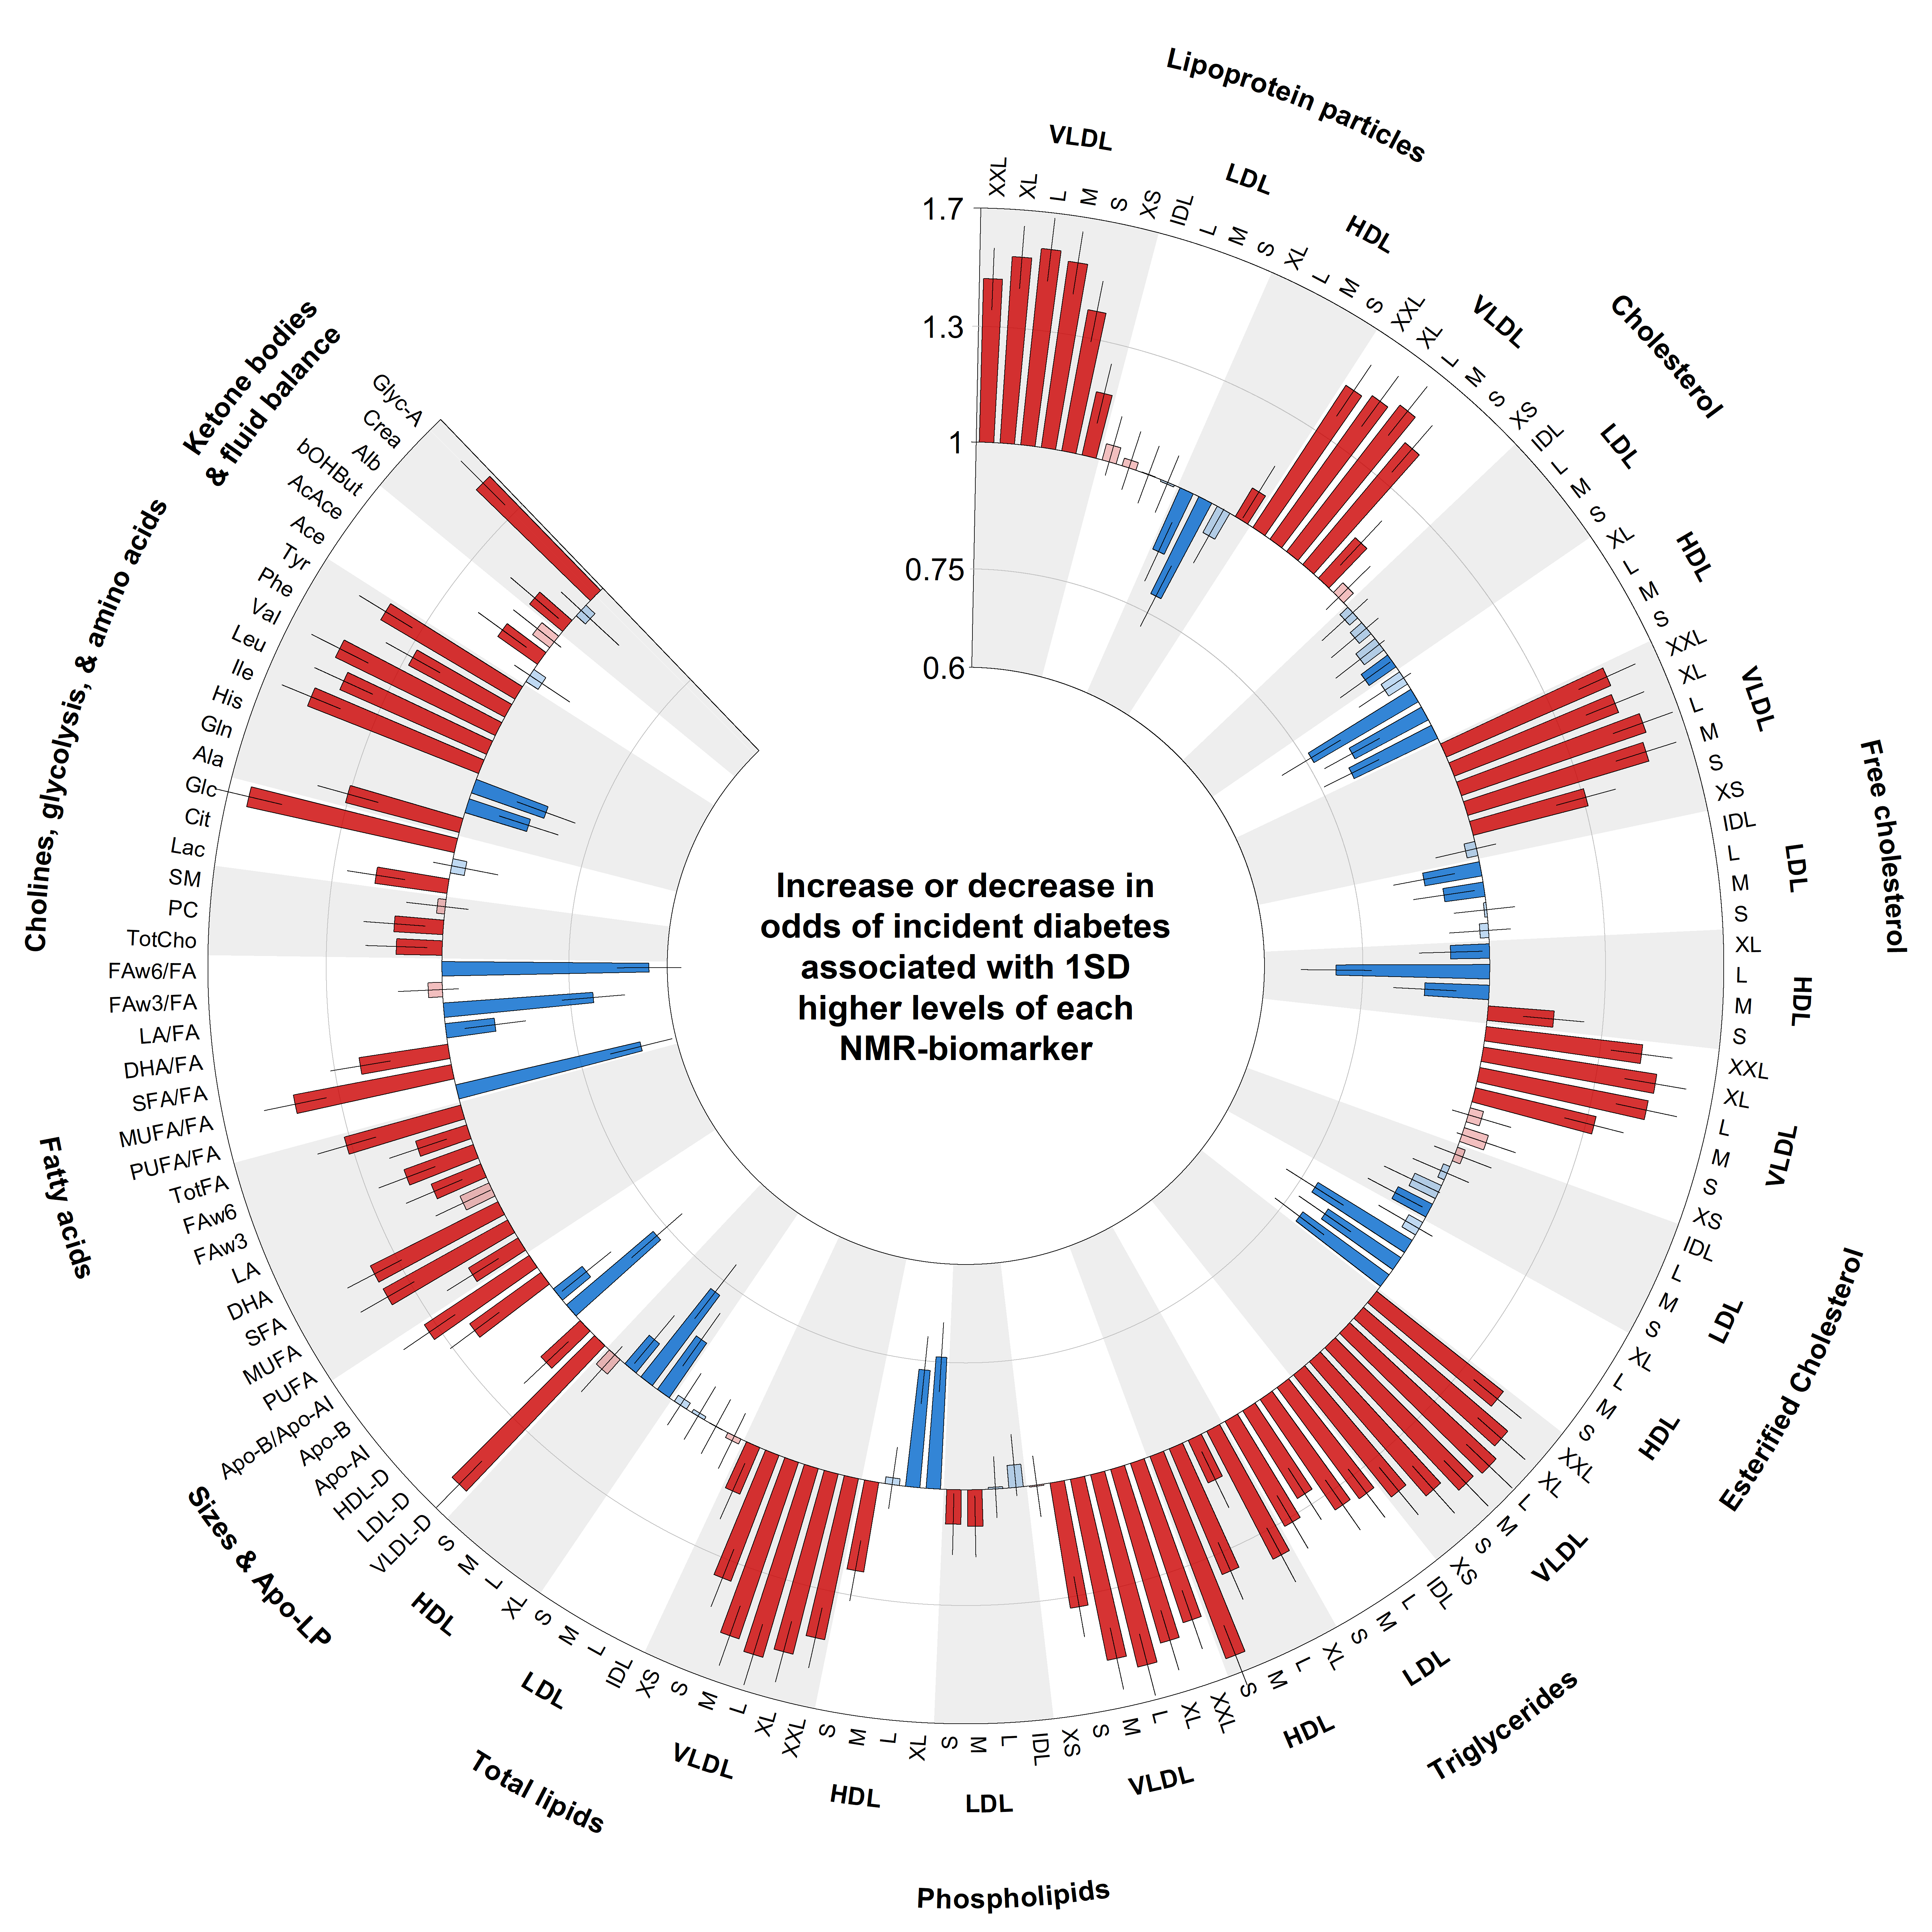
\includegraphics{foo.png}

\end{document}
